\documentclass[11pt]{article}

% Shared notes settings for Applied Machine Learning lectures (UPES).
% Keep this file free of \documentclass to allow reuse via \input.

\usepackage[utf8]{inputenc}
\usepackage[T1]{fontenc}
\usepackage{lmodern}          % scalable T1 fonts; without this pdflatex falls back
\input{glyphtounicode}        % to bitmapped EC Type 3 and the PDFs are neither
\pdfgentounicode=1            % searchable nor screen-reader friendly
\usepackage[a4paper,margin=1in]{geometry}
\usepackage{hyperref}
\usepackage{xurl}
\usepackage{booktabs}
\usepackage{amsmath}
\usepackage{amssymb}
\usepackage{listings}
\usepackage{xcolor}
\usepackage{enumitem}
\usepackage{parskip}

% Code listings (Python-oriented for this subject).
\lstset{
  language=Python,
  basicstyle=\ttfamily\small,
  keywordstyle=\color{blue},
  commentstyle=\color{gray},
  stringstyle=\color{teal},
  showstringspaces=false,
  columns=fullflexible,
  frame=single,
  framerule=0.2pt,
  breaklines=true
}

\setlist[itemize]{topsep=0.3em,itemsep=0.2em}
\setlist[enumerate]{topsep=0.3em,itemsep=0.2em}

% Simple per-section source line.
\newcommand{\notesources}[1]{\par\noindent{\small\color{gray}\textit{Sources:} \sloppy #1\par}}

% Unit-wise source strings for this subject (used by slides + notes).
% Path is relative to the lecture `latex/` folder (the compilation CWD).
\IfFileExists{../../../_shared/aml-sources.tex}{%
  % Source strings for Applied Machine Learning (CSAI2017P) — used by slides + notes.
% Prescribed texts and reference books are taken from the course syllabus.
% Support texts are the author-hosted open-access editions:
%   statlearning.com            (ISL with Python)
%   probml.github.io/pml-book   (Murphy, Probabilistic Machine Learning)
%   d2l.ai                      (Dive into Deep Learning)
%   mml-book.github.io          (Mathematics for Machine Learning)

\newcommand{\AMLRepoURL}{https://github.com/tali7c/Applied-Machine-Learning}

% --- prescribed -------------------------------------------------------------
\newcommand{\AMLPrescribed}{%
M\"uller and Guido, \textit{Introduction to Machine Learning with Python}, O'Reilly, 2016.;%
Bishop, \textit{Pattern Recognition and Machine Learning}, Springer, 2006.;%
Murphy, \textit{Machine Learning: A Probabilistic Perspective}, MIT Press, 2012.;%
Han, Kamber and Pei, \textit{Data Mining: Concepts and Techniques} (3e), Morgan Kaufmann, 2012.%
}

% --- unit-wise ---------------------------------------------------------------
\newcommand{\AMLUnitISources}{%
M\"uller and Guido, \textit{Introduction to Machine Learning with Python}, Ch. 1.;%
Bishop, \textit{Pattern Recognition and Machine Learning}, Ch. 1.;%
Murphy, \textit{Probabilistic Machine Learning: An Introduction}, MIT Press, 2022, Ch. 1.;%
Mitchell, \textit{Machine Learning}, McGraw Hill, 1997, Ch. 1.;%
Scikit-learn documentation, accessed 2026-08-04.%
}

\newcommand{\AMLUnitIISources}{%
Bishop, \textit{Pattern Recognition and Machine Learning}, \S1.5, \S4.3, \S7.1.;%
Zhang, Lipton, Li and Smola, \textit{Dive into Deep Learning}, \S3.4.;%
Shalev-Shwartz and Ben-David, \textit{Understanding Machine Learning}, Ch. 15.;%
Murphy, \textit{Probabilistic Machine Learning: An Introduction}, Ch. 5.%
}

\newcommand{\AMLUnitIIISources}{%
Zhang, Lipton, Li and Smola, \textit{Dive into Deep Learning}, Ch. 12 (Optimization Algorithms).;%
Deisenroth, Faisal and Ong, \textit{Mathematics for Machine Learning}, Ch. 7.;%
Kingma and Ba, ``Adam: A Method for Stochastic Optimization,'' ICLR 2015.;%
Ruder, ``An overview of gradient descent optimization algorithms,'' arXiv:1609.04747, 2016.%
}

\newcommand{\AMLUnitIVSources}{%
Han, Kamber and Pei, \textit{Data Mining: Concepts and Techniques} (3e), Ch. 3.;%
M\"uller and Guido, \textit{Introduction to Machine Learning with Python}, Ch. 3--4.;%
James, Witten, Hastie, Tibshirani and Taylor, \textit{An Introduction to Statistical Learning with Python}, Ch. 5--6, 12.;%
Scikit-learn documentation (preprocessing, model selection), accessed 2026-08-04.%
}

\newcommand{\AMLUnitVSources}{%
James et al., \textit{An Introduction to Statistical Learning with Python}, Ch. 3--6.;%
Bishop, \textit{Pattern Recognition and Machine Learning}, Ch. 3.;%
Deisenroth, Faisal and Ong, \textit{Mathematics for Machine Learning}, Ch. 9.;%
M\"uller and Guido, \textit{Introduction to Machine Learning with Python}, \S2.3.%
}

\newcommand{\AMLUnitVISources}{%
Han, Kamber and Pei, \textit{Data Mining: Concepts and Techniques} (3e), Ch. 8--9.;%
James et al., \textit{An Introduction to Statistical Learning with Python}, Ch. 8--9.;%
Bishop, \textit{Pattern Recognition and Machine Learning}, Ch. 4--5, 7, 14.;%
Zhang et al., \textit{Dive into Deep Learning}, Ch. 5.%
}

\newcommand{\AMLUnitVIISources}{%
Han, Kamber and Pei, \textit{Data Mining: Concepts and Techniques} (3e), Ch. 10.;%
James et al., \textit{An Introduction to Statistical Learning with Python}, Ch. 12.;%
M\"uller and Guido, \textit{Introduction to Machine Learning with Python}, \S3.5.;%
Ester, Kriegel, Sander and Xu, ``A density-based algorithm for discovering clusters (DBSCAN),'' KDD 1996.%
}

\newcommand{\AMLLabSources}{%
M\"uller and Guido, \textit{Introduction to Machine Learning with Python}, companion notebooks.;%
McKinney, \textit{Python for Data Analysis} (3e), O'Reilly, 2022.;%
Scikit-learn user guide, accessed 2026-08-04.;%
Matplotlib and Seaborn documentation, accessed 2026-08-04.%
}
%
}{%
  % Faculty copies live under `private/` so their compile CWD is different.
  \IfFileExists{../../../../public/_shared/aml-sources.tex}{%
    % Source strings for Applied Machine Learning (CSAI2017P) — used by slides + notes.
% Prescribed texts and reference books are taken from the course syllabus.
% Support texts are the author-hosted open-access editions:
%   statlearning.com            (ISL with Python)
%   probml.github.io/pml-book   (Murphy, Probabilistic Machine Learning)
%   d2l.ai                      (Dive into Deep Learning)
%   mml-book.github.io          (Mathematics for Machine Learning)

\newcommand{\AMLRepoURL}{https://github.com/tali7c/Applied-Machine-Learning}

% --- prescribed -------------------------------------------------------------
\newcommand{\AMLPrescribed}{%
M\"uller and Guido, \textit{Introduction to Machine Learning with Python}, O'Reilly, 2016.;%
Bishop, \textit{Pattern Recognition and Machine Learning}, Springer, 2006.;%
Murphy, \textit{Machine Learning: A Probabilistic Perspective}, MIT Press, 2012.;%
Han, Kamber and Pei, \textit{Data Mining: Concepts and Techniques} (3e), Morgan Kaufmann, 2012.%
}

% --- unit-wise ---------------------------------------------------------------
\newcommand{\AMLUnitISources}{%
M\"uller and Guido, \textit{Introduction to Machine Learning with Python}, Ch. 1.;%
Bishop, \textit{Pattern Recognition and Machine Learning}, Ch. 1.;%
Murphy, \textit{Probabilistic Machine Learning: An Introduction}, MIT Press, 2022, Ch. 1.;%
Mitchell, \textit{Machine Learning}, McGraw Hill, 1997, Ch. 1.;%
Scikit-learn documentation, accessed 2026-08-04.%
}

\newcommand{\AMLUnitIISources}{%
Bishop, \textit{Pattern Recognition and Machine Learning}, \S1.5, \S4.3, \S7.1.;%
Zhang, Lipton, Li and Smola, \textit{Dive into Deep Learning}, \S3.4.;%
Shalev-Shwartz and Ben-David, \textit{Understanding Machine Learning}, Ch. 15.;%
Murphy, \textit{Probabilistic Machine Learning: An Introduction}, Ch. 5.%
}

\newcommand{\AMLUnitIIISources}{%
Zhang, Lipton, Li and Smola, \textit{Dive into Deep Learning}, Ch. 12 (Optimization Algorithms).;%
Deisenroth, Faisal and Ong, \textit{Mathematics for Machine Learning}, Ch. 7.;%
Kingma and Ba, ``Adam: A Method for Stochastic Optimization,'' ICLR 2015.;%
Ruder, ``An overview of gradient descent optimization algorithms,'' arXiv:1609.04747, 2016.%
}

\newcommand{\AMLUnitIVSources}{%
Han, Kamber and Pei, \textit{Data Mining: Concepts and Techniques} (3e), Ch. 3.;%
M\"uller and Guido, \textit{Introduction to Machine Learning with Python}, Ch. 3--4.;%
James, Witten, Hastie, Tibshirani and Taylor, \textit{An Introduction to Statistical Learning with Python}, Ch. 5--6, 12.;%
Scikit-learn documentation (preprocessing, model selection), accessed 2026-08-04.%
}

\newcommand{\AMLUnitVSources}{%
James et al., \textit{An Introduction to Statistical Learning with Python}, Ch. 3--6.;%
Bishop, \textit{Pattern Recognition and Machine Learning}, Ch. 3.;%
Deisenroth, Faisal and Ong, \textit{Mathematics for Machine Learning}, Ch. 9.;%
M\"uller and Guido, \textit{Introduction to Machine Learning with Python}, \S2.3.%
}

\newcommand{\AMLUnitVISources}{%
Han, Kamber and Pei, \textit{Data Mining: Concepts and Techniques} (3e), Ch. 8--9.;%
James et al., \textit{An Introduction to Statistical Learning with Python}, Ch. 8--9.;%
Bishop, \textit{Pattern Recognition and Machine Learning}, Ch. 4--5, 7, 14.;%
Zhang et al., \textit{Dive into Deep Learning}, Ch. 5.%
}

\newcommand{\AMLUnitVIISources}{%
Han, Kamber and Pei, \textit{Data Mining: Concepts and Techniques} (3e), Ch. 10.;%
James et al., \textit{An Introduction to Statistical Learning with Python}, Ch. 12.;%
M\"uller and Guido, \textit{Introduction to Machine Learning with Python}, \S3.5.;%
Ester, Kriegel, Sander and Xu, ``A density-based algorithm for discovering clusters (DBSCAN),'' KDD 1996.%
}

\newcommand{\AMLLabSources}{%
M\"uller and Guido, \textit{Introduction to Machine Learning with Python}, companion notebooks.;%
McKinney, \textit{Python for Data Analysis} (3e), O'Reilly, 2022.;%
Scikit-learn user guide, accessed 2026-08-04.;%
Matplotlib and Seaborn documentation, accessed 2026-08-04.%
}
%
  }{%
    % Question papers live at `private/<family>/<instrument>/`.
    \IfFileExists{../../../public/_shared/aml-sources.tex}{%
      % Source strings for Applied Machine Learning (CSAI2017P) — used by slides + notes.
% Prescribed texts and reference books are taken from the course syllabus.
% Support texts are the author-hosted open-access editions:
%   statlearning.com            (ISL with Python)
%   probml.github.io/pml-book   (Murphy, Probabilistic Machine Learning)
%   d2l.ai                      (Dive into Deep Learning)
%   mml-book.github.io          (Mathematics for Machine Learning)

\newcommand{\AMLRepoURL}{https://github.com/tali7c/Applied-Machine-Learning}

% --- prescribed -------------------------------------------------------------
\newcommand{\AMLPrescribed}{%
M\"uller and Guido, \textit{Introduction to Machine Learning with Python}, O'Reilly, 2016.;%
Bishop, \textit{Pattern Recognition and Machine Learning}, Springer, 2006.;%
Murphy, \textit{Machine Learning: A Probabilistic Perspective}, MIT Press, 2012.;%
Han, Kamber and Pei, \textit{Data Mining: Concepts and Techniques} (3e), Morgan Kaufmann, 2012.%
}

% --- unit-wise ---------------------------------------------------------------
\newcommand{\AMLUnitISources}{%
M\"uller and Guido, \textit{Introduction to Machine Learning with Python}, Ch. 1.;%
Bishop, \textit{Pattern Recognition and Machine Learning}, Ch. 1.;%
Murphy, \textit{Probabilistic Machine Learning: An Introduction}, MIT Press, 2022, Ch. 1.;%
Mitchell, \textit{Machine Learning}, McGraw Hill, 1997, Ch. 1.;%
Scikit-learn documentation, accessed 2026-08-04.%
}

\newcommand{\AMLUnitIISources}{%
Bishop, \textit{Pattern Recognition and Machine Learning}, \S1.5, \S4.3, \S7.1.;%
Zhang, Lipton, Li and Smola, \textit{Dive into Deep Learning}, \S3.4.;%
Shalev-Shwartz and Ben-David, \textit{Understanding Machine Learning}, Ch. 15.;%
Murphy, \textit{Probabilistic Machine Learning: An Introduction}, Ch. 5.%
}

\newcommand{\AMLUnitIIISources}{%
Zhang, Lipton, Li and Smola, \textit{Dive into Deep Learning}, Ch. 12 (Optimization Algorithms).;%
Deisenroth, Faisal and Ong, \textit{Mathematics for Machine Learning}, Ch. 7.;%
Kingma and Ba, ``Adam: A Method for Stochastic Optimization,'' ICLR 2015.;%
Ruder, ``An overview of gradient descent optimization algorithms,'' arXiv:1609.04747, 2016.%
}

\newcommand{\AMLUnitIVSources}{%
Han, Kamber and Pei, \textit{Data Mining: Concepts and Techniques} (3e), Ch. 3.;%
M\"uller and Guido, \textit{Introduction to Machine Learning with Python}, Ch. 3--4.;%
James, Witten, Hastie, Tibshirani and Taylor, \textit{An Introduction to Statistical Learning with Python}, Ch. 5--6, 12.;%
Scikit-learn documentation (preprocessing, model selection), accessed 2026-08-04.%
}

\newcommand{\AMLUnitVSources}{%
James et al., \textit{An Introduction to Statistical Learning with Python}, Ch. 3--6.;%
Bishop, \textit{Pattern Recognition and Machine Learning}, Ch. 3.;%
Deisenroth, Faisal and Ong, \textit{Mathematics for Machine Learning}, Ch. 9.;%
M\"uller and Guido, \textit{Introduction to Machine Learning with Python}, \S2.3.%
}

\newcommand{\AMLUnitVISources}{%
Han, Kamber and Pei, \textit{Data Mining: Concepts and Techniques} (3e), Ch. 8--9.;%
James et al., \textit{An Introduction to Statistical Learning with Python}, Ch. 8--9.;%
Bishop, \textit{Pattern Recognition and Machine Learning}, Ch. 4--5, 7, 14.;%
Zhang et al., \textit{Dive into Deep Learning}, Ch. 5.%
}

\newcommand{\AMLUnitVIISources}{%
Han, Kamber and Pei, \textit{Data Mining: Concepts and Techniques} (3e), Ch. 10.;%
James et al., \textit{An Introduction to Statistical Learning with Python}, Ch. 12.;%
M\"uller and Guido, \textit{Introduction to Machine Learning with Python}, \S3.5.;%
Ester, Kriegel, Sander and Xu, ``A density-based algorithm for discovering clusters (DBSCAN),'' KDD 1996.%
}

\newcommand{\AMLLabSources}{%
M\"uller and Guido, \textit{Introduction to Machine Learning with Python}, companion notebooks.;%
McKinney, \textit{Python for Data Analysis} (3e), O'Reilly, 2022.;%
Scikit-learn user guide, accessed 2026-08-04.;%
Matplotlib and Seaborn documentation, accessed 2026-08-04.%
}
%
    }{%
      % Marking schemes live at `private/solutions/<family>/<id>/latex/`.
      \IfFileExists{../../../../../public/_shared/aml-sources.tex}{%
        % Source strings for Applied Machine Learning (CSAI2017P) — used by slides + notes.
% Prescribed texts and reference books are taken from the course syllabus.
% Support texts are the author-hosted open-access editions:
%   statlearning.com            (ISL with Python)
%   probml.github.io/pml-book   (Murphy, Probabilistic Machine Learning)
%   d2l.ai                      (Dive into Deep Learning)
%   mml-book.github.io          (Mathematics for Machine Learning)

\newcommand{\AMLRepoURL}{https://github.com/tali7c/Applied-Machine-Learning}

% --- prescribed -------------------------------------------------------------
\newcommand{\AMLPrescribed}{%
M\"uller and Guido, \textit{Introduction to Machine Learning with Python}, O'Reilly, 2016.;%
Bishop, \textit{Pattern Recognition and Machine Learning}, Springer, 2006.;%
Murphy, \textit{Machine Learning: A Probabilistic Perspective}, MIT Press, 2012.;%
Han, Kamber and Pei, \textit{Data Mining: Concepts and Techniques} (3e), Morgan Kaufmann, 2012.%
}

% --- unit-wise ---------------------------------------------------------------
\newcommand{\AMLUnitISources}{%
M\"uller and Guido, \textit{Introduction to Machine Learning with Python}, Ch. 1.;%
Bishop, \textit{Pattern Recognition and Machine Learning}, Ch. 1.;%
Murphy, \textit{Probabilistic Machine Learning: An Introduction}, MIT Press, 2022, Ch. 1.;%
Mitchell, \textit{Machine Learning}, McGraw Hill, 1997, Ch. 1.;%
Scikit-learn documentation, accessed 2026-08-04.%
}

\newcommand{\AMLUnitIISources}{%
Bishop, \textit{Pattern Recognition and Machine Learning}, \S1.5, \S4.3, \S7.1.;%
Zhang, Lipton, Li and Smola, \textit{Dive into Deep Learning}, \S3.4.;%
Shalev-Shwartz and Ben-David, \textit{Understanding Machine Learning}, Ch. 15.;%
Murphy, \textit{Probabilistic Machine Learning: An Introduction}, Ch. 5.%
}

\newcommand{\AMLUnitIIISources}{%
Zhang, Lipton, Li and Smola, \textit{Dive into Deep Learning}, Ch. 12 (Optimization Algorithms).;%
Deisenroth, Faisal and Ong, \textit{Mathematics for Machine Learning}, Ch. 7.;%
Kingma and Ba, ``Adam: A Method for Stochastic Optimization,'' ICLR 2015.;%
Ruder, ``An overview of gradient descent optimization algorithms,'' arXiv:1609.04747, 2016.%
}

\newcommand{\AMLUnitIVSources}{%
Han, Kamber and Pei, \textit{Data Mining: Concepts and Techniques} (3e), Ch. 3.;%
M\"uller and Guido, \textit{Introduction to Machine Learning with Python}, Ch. 3--4.;%
James, Witten, Hastie, Tibshirani and Taylor, \textit{An Introduction to Statistical Learning with Python}, Ch. 5--6, 12.;%
Scikit-learn documentation (preprocessing, model selection), accessed 2026-08-04.%
}

\newcommand{\AMLUnitVSources}{%
James et al., \textit{An Introduction to Statistical Learning with Python}, Ch. 3--6.;%
Bishop, \textit{Pattern Recognition and Machine Learning}, Ch. 3.;%
Deisenroth, Faisal and Ong, \textit{Mathematics for Machine Learning}, Ch. 9.;%
M\"uller and Guido, \textit{Introduction to Machine Learning with Python}, \S2.3.%
}

\newcommand{\AMLUnitVISources}{%
Han, Kamber and Pei, \textit{Data Mining: Concepts and Techniques} (3e), Ch. 8--9.;%
James et al., \textit{An Introduction to Statistical Learning with Python}, Ch. 8--9.;%
Bishop, \textit{Pattern Recognition and Machine Learning}, Ch. 4--5, 7, 14.;%
Zhang et al., \textit{Dive into Deep Learning}, Ch. 5.%
}

\newcommand{\AMLUnitVIISources}{%
Han, Kamber and Pei, \textit{Data Mining: Concepts and Techniques} (3e), Ch. 10.;%
James et al., \textit{An Introduction to Statistical Learning with Python}, Ch. 12.;%
M\"uller and Guido, \textit{Introduction to Machine Learning with Python}, \S3.5.;%
Ester, Kriegel, Sander and Xu, ``A density-based algorithm for discovering clusters (DBSCAN),'' KDD 1996.%
}

\newcommand{\AMLLabSources}{%
M\"uller and Guido, \textit{Introduction to Machine Learning with Python}, companion notebooks.;%
McKinney, \textit{Python for Data Analysis} (3e), O'Reilly, 2022.;%
Scikit-learn user guide, accessed 2026-08-04.;%
Matplotlib and Seaborn documentation, accessed 2026-08-04.%
}
%
      }{%
        % Source strings for Applied Machine Learning (CSAI2017P) — used by slides + notes.
% Prescribed texts and reference books are taken from the course syllabus.
% Support texts are the author-hosted open-access editions:
%   statlearning.com            (ISL with Python)
%   probml.github.io/pml-book   (Murphy, Probabilistic Machine Learning)
%   d2l.ai                      (Dive into Deep Learning)
%   mml-book.github.io          (Mathematics for Machine Learning)

\newcommand{\AMLRepoURL}{https://github.com/tali7c/Applied-Machine-Learning}

% --- prescribed -------------------------------------------------------------
\newcommand{\AMLPrescribed}{%
M\"uller and Guido, \textit{Introduction to Machine Learning with Python}, O'Reilly, 2016.;%
Bishop, \textit{Pattern Recognition and Machine Learning}, Springer, 2006.;%
Murphy, \textit{Machine Learning: A Probabilistic Perspective}, MIT Press, 2012.;%
Han, Kamber and Pei, \textit{Data Mining: Concepts and Techniques} (3e), Morgan Kaufmann, 2012.%
}

% --- unit-wise ---------------------------------------------------------------
\newcommand{\AMLUnitISources}{%
M\"uller and Guido, \textit{Introduction to Machine Learning with Python}, Ch. 1.;%
Bishop, \textit{Pattern Recognition and Machine Learning}, Ch. 1.;%
Murphy, \textit{Probabilistic Machine Learning: An Introduction}, MIT Press, 2022, Ch. 1.;%
Mitchell, \textit{Machine Learning}, McGraw Hill, 1997, Ch. 1.;%
Scikit-learn documentation, accessed 2026-08-04.%
}

\newcommand{\AMLUnitIISources}{%
Bishop, \textit{Pattern Recognition and Machine Learning}, \S1.5, \S4.3, \S7.1.;%
Zhang, Lipton, Li and Smola, \textit{Dive into Deep Learning}, \S3.4.;%
Shalev-Shwartz and Ben-David, \textit{Understanding Machine Learning}, Ch. 15.;%
Murphy, \textit{Probabilistic Machine Learning: An Introduction}, Ch. 5.%
}

\newcommand{\AMLUnitIIISources}{%
Zhang, Lipton, Li and Smola, \textit{Dive into Deep Learning}, Ch. 12 (Optimization Algorithms).;%
Deisenroth, Faisal and Ong, \textit{Mathematics for Machine Learning}, Ch. 7.;%
Kingma and Ba, ``Adam: A Method for Stochastic Optimization,'' ICLR 2015.;%
Ruder, ``An overview of gradient descent optimization algorithms,'' arXiv:1609.04747, 2016.%
}

\newcommand{\AMLUnitIVSources}{%
Han, Kamber and Pei, \textit{Data Mining: Concepts and Techniques} (3e), Ch. 3.;%
M\"uller and Guido, \textit{Introduction to Machine Learning with Python}, Ch. 3--4.;%
James, Witten, Hastie, Tibshirani and Taylor, \textit{An Introduction to Statistical Learning with Python}, Ch. 5--6, 12.;%
Scikit-learn documentation (preprocessing, model selection), accessed 2026-08-04.%
}

\newcommand{\AMLUnitVSources}{%
James et al., \textit{An Introduction to Statistical Learning with Python}, Ch. 3--6.;%
Bishop, \textit{Pattern Recognition and Machine Learning}, Ch. 3.;%
Deisenroth, Faisal and Ong, \textit{Mathematics for Machine Learning}, Ch. 9.;%
M\"uller and Guido, \textit{Introduction to Machine Learning with Python}, \S2.3.%
}

\newcommand{\AMLUnitVISources}{%
Han, Kamber and Pei, \textit{Data Mining: Concepts and Techniques} (3e), Ch. 8--9.;%
James et al., \textit{An Introduction to Statistical Learning with Python}, Ch. 8--9.;%
Bishop, \textit{Pattern Recognition and Machine Learning}, Ch. 4--5, 7, 14.;%
Zhang et al., \textit{Dive into Deep Learning}, Ch. 5.%
}

\newcommand{\AMLUnitVIISources}{%
Han, Kamber and Pei, \textit{Data Mining: Concepts and Techniques} (3e), Ch. 10.;%
James et al., \textit{An Introduction to Statistical Learning with Python}, Ch. 12.;%
M\"uller and Guido, \textit{Introduction to Machine Learning with Python}, \S3.5.;%
Ester, Kriegel, Sander and Xu, ``A density-based algorithm for discovering clusters (DBSCAN),'' KDD 1996.%
}

\newcommand{\AMLLabSources}{%
M\"uller and Guido, \textit{Introduction to Machine Learning with Python}, companion notebooks.;%
McKinney, \textit{Python for Data Analysis} (3e), O'Reilly, 2022.;%
Scikit-learn user guide, accessed 2026-08-04.;%
Matplotlib and Seaborn documentation, accessed 2026-08-04.%
}
%
      }%
    }%
  }%
}


\graphicspath{{../figures/}}

% This lecture pairs almost every paragraph with a listing and its output, so
% the default \medskipamount around each block adds up to several pages.
\lstset{aboveskip=3pt, belowskip=3pt}
\captionsetup{skip=3pt, font=small}
\tcbset{before skip=4pt, after skip=6pt}
% Eleven wide figures in a text-dense document: let them share pages with
% prose instead of being pushed onto float pages of their own.
\renewcommand{\topfraction}{0.92}
\renewcommand{\bottomfraction}{0.75}
\renewcommand{\textfraction}{0.06}
\renewcommand{\floatpagefraction}{0.85}
\setlength{\floatsep}{6pt plus 2pt minus 2pt}
\setlength{\textfloatsep}{8pt plus 2pt minus 2pt}
\setlength{\intextsep}{8pt plus 2pt minus 2pt}
% Long \texttt{} identifiers and URLs sit in ordinary prose throughout; give
% the line breaker room rather than accepting overfull boxes.
\setlength{\emergencystretch}{3.5em}
% Four algorithms in one set of notes: tighten the inter-paragraph glue a
% little so the document stays inside its page budget without cutting
% material.
\setlength{\parskip}{0.42\baselineskip plus 1pt minus 1pt}

\title{Applied Machine Learning\\Unit 07 --- Lecture 23 Notes\\
       Partitioning and Density-Based Clustering}
\author{Tofik Ali}
\date{Autumn 2026}

\begin{document}
\maketitle

\begin{keyidea}[Read this first]
These notes are written so that you can learn the material \emph{without}
having been in the lecture. Every concept is developed from scratch, every
number you see was produced by running the code shown beside it, and every
figure was generated from real computation rather than drawn by hand.

The previous lecture built a whole family of clusterings at once, as a tree,
and left you to cut it. This lecture takes the opposite bargain twice over.
First, \textbf{partitioning}: you say how many clusters you want, and you get
exactly one partition, quickly, on data a tree could never fit in memory ---
at the price of having to know $k$ in advance and of getting a different
answer every time you run it. Then, \textbf{density-based clustering}: refuse
to name $k$, refuse to assume clusters are round, and allow the method to
say that a point belongs to nothing at all.

Two calculations carry this lecture and you must be able to do both with a
pen. The first is \textbf{a complete $k$-means run on seven points with
$k = 2$} (Section~\ref{sec:hand}): the distance table at every assignment
step, the means at every update step, and the objective after every half
step, falling $123 \to 32.2 \to 16.74 \to 11.4167$ until nothing moves. The
second is \textbf{eleven points labelled core, border or noise
arithmetically} (Section~\ref{sec:dbscan}), giving seven core points, two
border points, two noise points and two clusters --- with $k$ never supplied.
Both are then confirmed against \texttt{scikit-learn} exactly.

Four results are worth remembering a year from now. \textbf{$k$-means
converges, but only to a local optimum}: twenty random starts on one data set
give twelve different answers, the worst $11.6$ times the best
(Section~\ref{sec:conv}). \textbf{Two outliers in $302$ points} take
$k$-means from ARI $1.000$ to $0.000$ while $k$-medoids does not move
(Section~\ref{sec:medoid}). \textbf{CLARA does $1576$ times less work than
PAM} at $n = 4000$ for $4.4\%$ more cost (Section~\ref{sec:clara}). And
\textbf{no single $\varepsilon$ serves two densities} --- there is a data set
in Section~\ref{sec:eps} on which every value of $\varepsilon$ either
dissolves the loose cluster into noise or welds the two tight ones together.
\end{keyidea}

\tableofcontents
\medskip

% =========================================================================
\section{How to use these notes}
\label{sec:how}

Read in order. Sections~\ref{sec:part} to \ref{sec:conv} are one continuous
thread --- what the partitioning problem is, $k$-means run by hand, and why
it stops where it stops --- and nothing later makes sense without them.
Section~\ref{sec:k} is about choosing $k$ and is mostly a warning.
Section~\ref{sec:assume} is the honest account of what $k$-means assumes, and
it motivates everything after it: Sections~\ref{sec:medoid}
and~\ref{sec:clara} fix the \emph{robustness} and the \emph{scale} problems
while keeping the partitioning idea, and Sections~\ref{sec:dbscan}
and~\ref{sec:eps} throw the partitioning idea away entirely.
Section~\ref{sec:choose} puts the four methods in one table.

Everything here assumes the earlier clustering lectures: what clustering is
for, how a dissimilarity between two objects is defined, and how hierarchical
clustering works. If you cannot write down the Euclidean distance between two
rows and say what standardising does to it, read those first.

There are four kinds of box. \textbf{Key idea} --- the one sentence to
remember a month from now. \textbf{Worked example} --- a calculation done by
hand, with small numbers, before any library is used. \textbf{Caution} --- the
specific mistake that section exists to prevent. \textbf{Try it yourself} ---
something to run, with the expected output given so you can check.

Code appears in a framed block, and directly beneath it a shaded block showing
what that code \emph{actually printed}. If you run it and get something
different, trust your machine and tell me. Timings are the one exception:
those depend on your hardware, and only their \emph{ratios} and \emph{growth
rates} are meant to reproduce.

\subsection{What you need}

\begin{lstlisting}
pip install numpy scipy scikit-learn matplotlib
\end{lstlisting}

Every number in these notes was produced with:

\begin{lstlisting}
import numpy, scipy, sklearn, matplotlib
print("numpy", numpy.__version__, "| scipy", scipy.__version__,
      "| sklearn", sklearn.__version__,
      "| matplotlib", matplotlib.__version__)
\end{lstlisting}
\begin{codeout}
numpy 2.2.6 | scipy 1.15.3 | sklearn 1.7.2 | matplotlib 3.10.9
\end{codeout}

These imports appear everywhere below:

\begin{lstlisting}
import numpy as np
from scipy.spatial.distance import cdist, pdist, squareform
from sklearn.cluster import KMeans, DBSCAN
from sklearn.datasets import (load_iris, load_wine, load_breast_cancer,
                              load_digits, make_blobs, make_moons,
                              make_circles)
from sklearn.metrics import adjusted_rand_score, silhouette_score
from sklearn.neighbors import NearestNeighbors
from sklearn.preprocessing import StandardScaler
\end{lstlisting}

\begin{caution}[$k$-medoids is not in scikit-learn]
There is no \texttt{KMedoids} in \texttt{sklearn.cluster}. The usual answer is
the \texttt{scikit-learn-extra} package, which provides
\texttt{sklearn\_extra.cluster.KMedoids} (with \texttt{method="pam"}) and
\texttt{sklearn\_extra.cluster.CLARA}. It is \emph{not} installed in the lab
image, and the notes do not depend on it: Sections~\ref{sec:medoid}
and~\ref{sec:clara} implement PAM and CLARA from scratch in about forty lines.
That is better for learning anyway, because the SWAP step is then visible
rather than hidden behind a \texttt{fit} call.
\end{caution}

Four bundled datasets recur, and \textbf{none of them downloads anything}:
\texttt{load\_iris} ($150 \times 4$), \texttt{load\_wine} ($178 \times 13$),
\texttt{load\_breast\_cancer} ($569 \times 30$) and \texttt{load\_digits}
($1797 \times 64$). Everything else is a fixed-seed synthetic set --- blobs,
two moons, concentric circles, two long thin bands, and a three-cluster set
with deliberately mismatched densities.

\begin{caution}[Do not reach for \texttt{fetch\_*}]
Every \texttt{fetch\_*} loader downloads over HTTPS, and on the campus network
those downloads fail with a certificate error you cannot fix from your machine.
Nothing in this course depends on one: use the bundled loaders or a fixed-seed
synthetic set.
\end{caution}

\begin{keyidea}[Three kinds of seed, and this lecture uses all three]
More than any other lecture in the course, this one is \emph{about} random
seeds --- so it is worth being precise about which kind you are looking at
before you copy a line of code.

\textbf{One arbitrary seed, $0$.} Every \texttt{KMeans} start that is not part
of an experiment, every CLARA sampling run, every contamination draw:
\texttt{random\_state=0}, \texttt{np.random.default\_rng(0)}. It is arbitrary;
it is written down so that you get the same answer.

\textbf{Dataset seeds, which are not arbitrary at all.}
\texttt{make\_blobs(\dots, random\_state=7)} for the six blobs,
\texttt{random\_state=11} for the four clean ones, \texttt{random\_state=3} for
the very unequal sizes, and so on. These \emph{define the shape of the
problem}, and the shape is the argument the section is making. Change one and
you are no longer looking at the phenomenon.

\textbf{Sweep seeds, where the variation \emph{is} the result.} When
Section~\ref{sec:local} runs $k$-means from $200$ different starts, the
disagreement between those runs is the entire point: it is how you see that
Lloyd's algorithm converges to a \emph{local} optimum. Replacing
\texttt{for s in range(200)} with a single seed would not tidy the experiment
up, it would delete it.

\begin{center}
\textbf{And the practical warning: pin \texttt{n\_init} as well as
\texttt{random\_state}.}
\end{center}

\noindent \texttt{KMeans} has two independent sources of variation, and
fixing one is not enough. \texttt{random\_state} fixes \emph{where} the starts
come from; \texttt{n\_init} fixes \emph{how many} of them there are, and its
default is \texttt{"auto"} --- which is $1$ for \texttt{k-means++} and $10$
for \texttt{init="random"}, and which changed in scikit-learn~1.4. A student
who writes \texttt{KMeans(n\_clusters=6)} and nothing else will not reproduce
the figures in this lecture, and will not know why. Every listing below shows
both.
\end{keyidea}

\subsection{Learning outcomes}

These notes serve \textbf{CO4} --- \emph{apply and evaluate learning
techniques, and select an appropriate model for a given problem}. By the end
you should be able to:

\begin{enumerate}[leftmargin=*]
  \item State the partitioning clustering problem, write down the $k$-means
    objective, and explain why exhaustive search is not an option.
    \hfill \textbf{CO4}
  \item \textbf{Execute a complete $k$-means run by hand}: the distance table
    at each assignment step, the means at each update step, and the
    within-cluster sum of squares after every half step, until nothing
    changes. \hfill \textbf{CO4}
  \item Prove that both steps of Lloyd's algorithm are non-increasing in the
    objective, and use the finiteness of the set of partitions to argue that
    the algorithm terminates --- at a \emph{local} optimum. \hfill \textbf{CO4}
  \item Explain and quantify the effect of initialisation, describe
    $k$-means\texttt{++}, and choose \texttt{n\_init} for a given
    problem. \hfill \textbf{CO4}
  \item Apply the elbow and silhouette heuristics for choosing $k$, and state
    honestly what each one is and is not. \hfill \textbf{CO4}
  \item Name the three assumptions built into the $k$-means objective and
    identify data on which each of them fails. \hfill \textbf{CO4}
  \item Define the $k$-medoids objective, compute it for a given set of
    medoids, work a SWAP step, and explain why a medoid is more robust than a
    mean. \hfill \textbf{CO4}
  \item State the per-iteration complexity of PAM, explain the CLARA
    sampling scheme, and reason quantitatively about the time and quality
    trade-off. \hfill \textbf{CO4}
  \item \textbf{Classify every point of a small data set as core, border or
    noise} for given $\varepsilon$ and minPts, chain the core points into
    clusters, and identify the noise. \hfill \textbf{CO4}
  \item Explain why a single global $\varepsilon$ cannot serve clusters of
    different density, use the $k$-distance graph to choose $\varepsilon$, and
    say what it does and does not settle. \hfill \textbf{CO4}
  \item Choose between hierarchical, partitioning and density-based
    clustering for a stated problem and defend the choice. \hfill \textbf{CO4}
\end{enumerate}

% =========================================================================
\section{The partitioning problem}
\label{sec:part}

\subsection{One partition, and you have to ask for it}

A \textbf{partitioning} method is given $n$ objects and an integer $k$, and
returns a partition of the objects into exactly $k$ non-empty groups. That is
the whole contract. There is no tree, no sequence of nested clusterings, and
no way to look at the answer for $k = 4$ and then ask for $k = 5$ without
running the method again.

Compared with the hierarchical methods of the previous lecture, this is a
trade in both directions. You lose the ability to defer the choice of $k$, and
you lose determinism --- almost every partitioning algorithm in practical use
is randomised. What you gain is scale. A hierarchical method needs the
$n \times n$ proximity matrix; a partitioning method needs only the $n$ rows
and $k$ representatives, so it runs in linear memory, and $k$-means on
$200{,}000$ points takes under a third of a second.

\subsection{The $k$-means objective}

The criterion $k$-means optimises is the \textbf{within-cluster sum of
squares}, also called the \emph{inertia} or the \emph{distortion}:
\begin{equation}
  \mathrm{WCSS}(C_1,\ldots,C_k)
  \;=\; \sum_{j=1}^{k}\ \sum_{x \in C_j} \lVert x - c_j \rVert_2^2,
  \qquad
  c_j \;=\; \frac{1}{|C_j|}\sum_{x \in C_j} x .
  \label{eq:wcss}
\end{equation}

Three things in equation~\eqref{eq:wcss} deserve to be said out loud, because
almost every property of $k$-means follows from one of them.

\textbf{The distance is squared.} That is not a convenience. It is exactly
what makes the mean the optimal representative of a cluster
(Section~\ref{sec:conv} proves it), and it is what makes one distant point so
expensive: a point twice as far away costs four times as much, so the
objective will happily distort a whole cluster to accommodate it.

\textbf{The representative is a single point.} A cluster is therefore
described entirely by one location. The boundary between two clusters is the
perpendicular bisector of the segment joining their centroids, so every
cluster $k$-means can produce is a cell of a Voronoi diagram, and therefore
\textbf{convex}. No amount of tuning will make $k$-means return a crescent.

\textbf{The sum runs over points, not clusters.} A cluster with $400$ members
contributes $400$ terms and a cluster with $40$ contributes $40$. The
objective is therefore much more interested in the big cluster, and will
gladly split it in two if that buys more than leaving the small one intact.

\begin{keyidea}
$k$-means does not look for ``clusters''. It looks for the $k$ points that
minimise the total squared distance from every observation to its nearest
one. Everything the method does well, and everything it does badly, is a
consequence of that specific sentence.
\end{keyidea}

\subsection{Why not just try every partition?}

The obvious algorithm is to enumerate all partitions of $n$ objects into $k$
non-empty groups and keep the best. The number of them is the Stirling number
of the second kind,
\[
  S(n,k) = \frac{1}{k!}\sum_{i=0}^{k}(-1)^i\binom{k}{i}(k-i)^n ,
\]
which for $k = 2$ reduces to the pleasant $2^{n-1}-1$.

\begin{lstlisting}
from math import comb, factorial
def S(n, k):
    return sum((-1)**i * comb(k, i) * (k-i)**n
               for i in range(k+1)) // factorial(k)
for n, k in [(7,2), (10,3), (25,3), (50,5), (100,3)]:
    print(n, k, S(n, k))
\end{lstlisting}
\begin{codeout}
   n      k    partitions S(n,k)
     7      2    63
    10      3    9330
    25      3    1.41198e+11
    50      5    7.40096e+32
   100      3    8.58963e+46
\end{codeout}

On seven points with $k = 2$ there are $63$ partitions, and later in this
section we really will check all of them. On a hundred points with $k = 3$
there are $8.6 \times 10^{46}$, and the discussion is over. The $k$-means
problem is NP-hard --- for $k = 2$ in general dimension, and for general $k$
in the plane --- so nobody solves it. What everybody runs is a heuristic, and
the honest thing is to say so and then measure how badly it can fail.

But notice: the number is \emph{finite}. That is half of the termination
argument in Section~\ref{sec:conv}.

\subsection{Lloyd's algorithm}

The heuristic is due to Lloyd (1957, published 1982) and is what everybody
means by ``$k$-means'':

\begin{lstlisting}
Input : n points, an integer k, initial centroids c_1 ... c_k
Output: an assignment of every point to one of k clusters

repeat
    # ASSIGNMENT step
    for each point x:  assign x to the cluster j minimising ||x - c_j||
    # UPDATE step
    for each cluster j: c_j = mean of the points now assigned to j
until no point changes cluster
\end{lstlisting}

Two steps, alternating. Fix the centres and optimise the assignment; fix the
assignment and optimise the centres. Neither step ever has to consider the
other's problem, which is why the algorithm is four lines long and why it is
fast.

Note what is \emph{not} in the loop: no choice of $k$, no learning rate, no
convergence tolerance, no regularisation. There is exactly one free decision,
the initial centroids, and Section~\ref{sec:conv} shows that it decides the
answer.

% =========================================================================
\section{A complete $k$-means run, by hand}
\label{sec:hand}

This is the examinable calculation of the lecture. Work it with a pen at
least once before the assessment.

\subsection{The seven points}

\begin{center}
\begin{tabular}{lccccccc}
  \toprule
  & $P_1$ & $P_2$ & $P_3$ & $P_4$ & $P_5$ & $P_6$ & $P_7$ \\
  \midrule
  $x$ & 1 & 2 & 2 & 5 & 7 & 8 & 8 \\
  $y$ & 2 & 1 & 3 & 4 & 5 & 4 & 6 \\
  \bottomrule
\end{tabular}
\end{center}

Seven points on an integer grid, $k = 2$. The initial centroids are taken
from the data and chosen \emph{badly} on purpose: $c_1^{(0)} = P_1 = (1,2)$
and $c_2^{(0)} = P_3 = (2,3)$, both sitting in the left-hand clump.
Figure~\ref{fig:handpoints} shows the arrangement.

\begin{figure}[htbp]
  \centering
  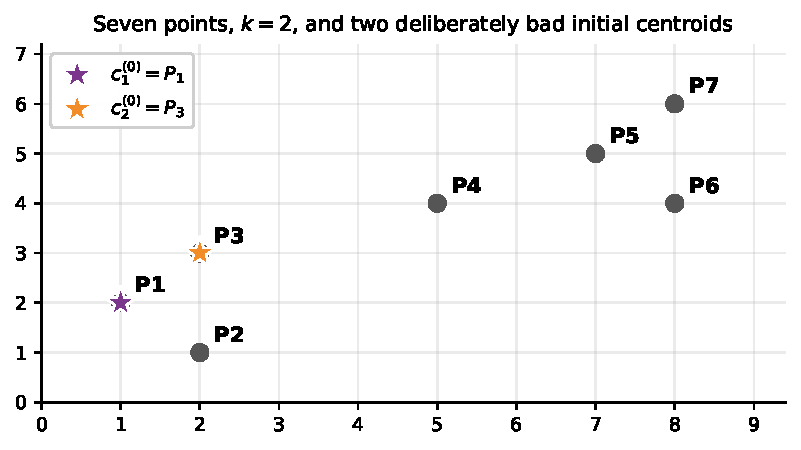
\includegraphics[width=0.68\textwidth]{handpoints.pdf}
  \caption{The seven points, and the two initial centroids. Both stars are in
    the left-hand group; the four right-hand points are nowhere near either.}
  \label{fig:handpoints}
\end{figure}

Choosing the initial centroids from the data is standard --- it guarantees
that no cluster starts empty --- and choosing them both on one side is what
makes the run interesting. A well-spread start would converge in two
iterations with nothing changing, and you would learn nothing.

\subsection{Iteration 1, assignment step}

For every point, compute the Euclidean distance to each centroid and assign it
to the smaller. With $c_1 = (1,2)$ and $c_2 = (2,3)$:

\begin{worked}[Iteration 1: the distance table]
\[
\begin{array}{lccl}
  \text{point} & d(\cdot, c_1) & d(\cdot, c_2) & \text{cluster}\\[2pt]
  P_1 (1,2) & \sqrt{0+0} = 0.0000 & \sqrt{1+1} = 1.4142 & C_1\\
  P_2 (2,1) & \sqrt{1+1} = 1.4142 & \sqrt{0+4} = 2.0000 & C_1\\
  P_3 (2,3) & \sqrt{1+1} = 1.4142 & \sqrt{0+0} = 0.0000 & C_2\\
  P_4 (5,4) & \sqrt{16+4} = 4.4721 & \sqrt{9+1} = 3.1623 & C_2\\
  P_5 (7,5) & \sqrt{36+9} = 6.7082 & \sqrt{25+4} = 5.3852 & C_2\\
  P_6 (8,4) & \sqrt{49+4} = 7.2801 & \sqrt{36+1} = 6.0828 & C_2\\
  P_7 (8,6) & \sqrt{49+16} = 8.0623 & \sqrt{36+9} = 6.7082 & C_2
\end{array}
\]
So $C_1 = \{P_1, P_2\}$ and $C_2 = \{P_3,P_4,P_5,P_6,P_7\}$.
\end{worked}

The objective at this point is computed with the \emph{current} centroids,
which are still $(1,2)$ and $(2,3)$:
\[
  \mathrm{WCSS} = \underbrace{0 + 2}_{C_1}
  + \underbrace{0 + 10 + 29 + 37 + 45}_{C_2} = 2 + 121 = 123.0000 .
\]
(Each term is the \emph{squared} distance: $1.4142^2 = 2$, $3.1623^2 = 10$,
and so on.)

\subsection{Iteration 1, update step}

Each centroid moves to the mean of the points now assigned to it:
\[
  c_1 = \tfrac12\bigl(1{+}2,\; 2{+}1\bigr) = (1.5,\ 1.5),
  \qquad
  c_2 = \tfrac15\bigl(30,\; 22\bigr) = (6.0,\ 4.4),
\]
where $30 = 2{+}5{+}7{+}8{+}8$ and $22 = 3{+}4{+}5{+}4{+}6$.
Recompute the objective with the same assignment and the new centres:
\[
  \mathrm{WCSS} = \underbrace{0.5 + 0.5}_{C_1}
  + \underbrace{17.96 + 1.16 + 1.36 + 4.16 + 6.56}_{C_2}
  = 1.0 + 31.2 = 32.2000 .
\]

Nothing was reassigned, and the objective fell from $123$ to $32.2$ purely
because the two centres moved to the means of their clusters. That is the
entire purpose of the update step, and it is worth pausing on: \emph{half} of
$k$-means' progress at this iteration came from moving points, and half from
moving centres.

\subsection{Iteration 2}

\begin{worked}[Iteration 2: one point crosses over]
With $c_1 = (1.5, 1.5)$ and $c_2 = (6.0, 4.4)$:
\[
\begin{array}{lccl}
  \text{point} & d(\cdot, c_1) & d(\cdot, c_2) & \text{cluster}\\[2pt]
  P_1 (1,2) & 0.7071 & 5.5462 & C_1\\
  P_2 (2,1) & 0.7071 & 5.2498 & C_1\\
  P_3 (2,3) & \mathbf{1.5811} & \mathbf{4.2379} & \mathbf{C_1 \text{ --- moved}}\\
  P_4 (5,4) & 4.3012 & 1.0770 & C_2\\
  P_5 (7,5) & 6.5192 & 1.1662 & C_2\\
  P_6 (8,4) & 6.9642 & 2.0396 & C_2\\
  P_7 (8,6) & 7.9057 & 2.5612 & C_2
\end{array}
\]
The two numbers that matter are
$d(P_3, c_1) = \sqrt{0.5^2 + 1.5^2} = \sqrt{2.5} = 1.5811$ and
$d(P_3, c_2) = \sqrt{4^2 + 1.4^2} = \sqrt{17.96} = 4.2379$.
\end{worked}

$P_3$ was only in $C_2$ because $c_2$ \emph{started} on top of it. One update
step later, $c_2$ has been dragged to $(6, 4.4)$ by the four right-hand
points, and $P_3$ is left behind.

The objective with the new assignment and the old centres is
\[
  \mathrm{WCSS} = (0.5 + 0.5 + 2.5) + (1.16 + 1.36 + 4.16 + 6.56)
  = 3.5 + 13.24 = 16.7400 ,
\]
and after the update step, with
$c_1 = \bigl(\tfrac53, 2\bigr) = (1.6667,\ 2.0000)$ and
$c_2 = (7.0000,\ 4.7500)$,
\[
  \mathrm{WCSS} = \underbrace{\tfrac{8}{3}}_{C_1}
  + \underbrace{\tfrac{35}{4}}_{C_2}
  = \tfrac{32}{12} + \tfrac{105}{12} = \tfrac{137}{12} = 11.4167 .
\]

\subsection{Iteration 3: nothing moves}

\begin{codeout}
  point      coord      d(.,c1)   d(.,c2)   cluster
  P1     ( 1.0, 2.0)    0.6667    6.6002   C1
  P2     ( 2.0, 1.0)    1.0541    6.2500   C1
  P3     ( 2.0, 3.0)    1.0541    5.2974   C1
  P4     ( 5.0, 4.0)    3.8873    2.1360   C2
  P5     ( 7.0, 5.0)    6.1192    0.2500   C2
  P6     ( 8.0, 4.0)    6.6416    1.2500   C2
  P7     ( 8.0, 6.0)    7.4907    1.6008   C2
  clusters: C1 = {P1,P2,P3}   C2 = {P4,P5,P6,P7}
  WCSS after assignment = 11.4167
  no point changed cluster -- CONVERGED after 3 iterations
\end{codeout}

Every point is already with its nearest centroid, so the assignment step
changes nothing, so the update step would change nothing, so the algorithm
stops. Figure~\ref{fig:handrun} shows all five half steps.

\begin{figure}[htbp]
  \centering
  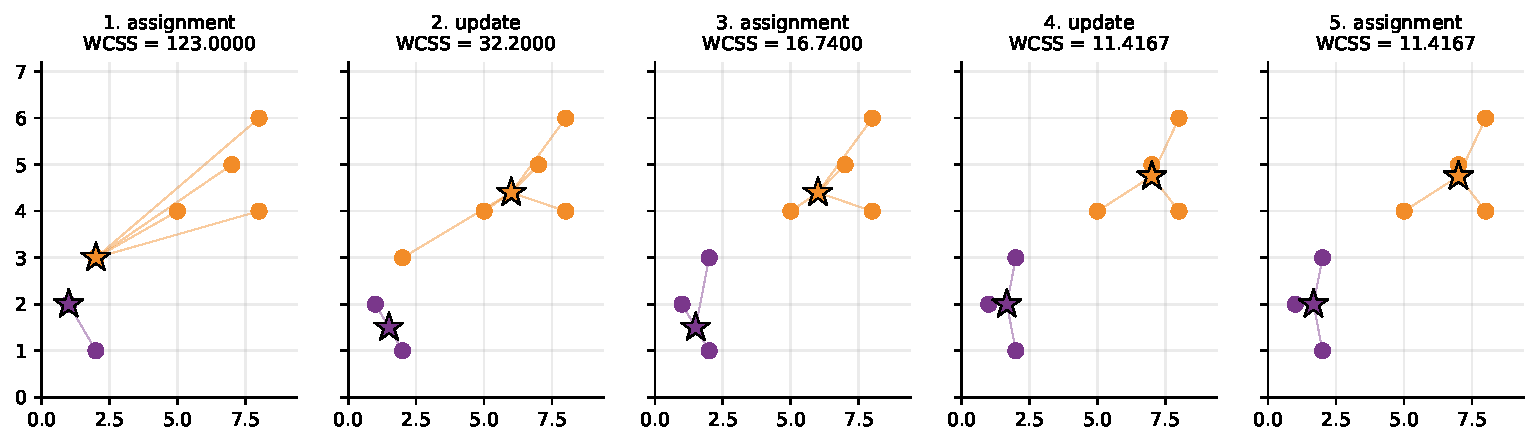
\includegraphics[width=\textwidth]{handrun.pdf}
  \caption{The complete run. Stars are centroids and the thin lines are the
    distances the objective sums. The panels alternate assignment, update,
    assignment, update, assignment --- and the last panel is identical to the
    fourth, which is what convergence means.}
  \label{fig:handrun}
\end{figure}

\subsection{The library agrees, exactly}

\begin{lstlisting}
P7 = np.array([[1.,2.],[2.,1.],[2.,3.],[5.,4.],[7.,5.],[8.,4.],[8.,6.]])
km = KMeans(n_clusters=2, init=np.array([P7[0], P7[2]]),
            n_init=1, algorithm="lloyd").fit(P7)
print(km.labels_, km.cluster_centers_, km.inertia_, km.n_iter_)
\end{lstlisting}
\begin{codeout}
sklearn labels    [0 0 0 1 1 1 1]
hand labels       [0 0 0 1 1 1 1]
sklearn centres   [[1.6667, 2.0], [7.0, 4.75]]
hand centres      [[1.6667, 2.0], [7.0, 4.75]]
sklearn inertia_ 11.416667
hand WCSS        11.416667
match to 1e-12:   True
iterations n_iter_ = 3
\end{codeout}

Passing \texttt{init} an explicit array and \texttt{n\_init=1} is how you make
scikit-learn run the algorithm you just did by hand rather than its own
$k$-means\texttt{++} restarts. \texttt{inertia\_} is exactly
equation~\eqref{eq:wcss}, and \texttt{n\_iter\_} counts the iterations the
same way we did.

\subsection{Was that the global optimum?}

On seven points we can simply check. There are $2^{6} - 1 = 63$ ways to split
them into two non-empty groups.

\begin{lstlisting}
best = None
for mask in range(1, 2**(len(P7)-1)):
    m = np.array([(mask >> i) & 1 for i in range(len(P7))])
    if 0 < m.sum() < len(P7):
        cs = np.array([P7[m == 0].mean(axis=0), P7[m == 1].mean(axis=0)])
        w = wcss(P7, m, cs)
        if best is None or w < best[0]: best = (w, m.copy())
print(best[0])
\end{lstlisting}
\begin{codeout}
partitions examined: 2^(n-1) - 1 = 63
best WCSS over all partitions = 11.4167
best partition: C1 = {P4,P5,P6,P7}  C2 = {P1,P2,P3}
Lloyd from (P1,P3) found it: True
\end{codeout}

\begin{caution}[Do not generalise from seven points]
Lloyd's algorithm found the global optimum here from a deliberately bad
start. That is a property of a tiny, clean, well-separated example. The very
next section exhibits a data set on which twenty different random starts give
twelve different answers, the worst of them $11.6$ times worse than the best.
\end{caution}

% =========================================================================
\section{Why it converges, and to what}
\label{sec:conv}

\subsection{The termination argument}

\begin{keyidea}
Each of the two steps can only lower the objective, and there are finitely
many partitions, so the algorithm must stop. Nothing in that argument says
anything about \emph{where} it stops.
\end{keyidea}

\textbf{Step 1: the assignment step cannot increase WCSS.} With the centres
held fixed, each point's contribution to equation~\eqref{eq:wcss} is
$\lVert x - c_{j(x)}\rVert^2$ for whatever cluster $j(x)$ it currently belongs
to. Reassigning it to the nearest centre replaces this by
$\min_j \lVert x - c_j\rVert^2$, which is at most as large. Sum over points.

\textbf{Step 2: the update step cannot increase WCSS.} This needs the
following small lemma, which is the reason $k$-means uses the mean and not
something else.

\begin{worked}[The mean minimises the sum of squared distances]
For any finite set $S$ with mean $\bar{x} = \frac{1}{|S|}\sum_{x \in S} x$ and
any point $z$,
\begin{equation}
  \sum_{x \in S}\lVert x - z\rVert^2
  = \sum_{x \in S}\lVert x - \bar{x}\rVert^2 + |S|\,\lVert \bar{x} - z\rVert^2 .
  \label{eq:meanlemma}
\end{equation}
\emph{Proof.} Write $x - z = (x - \bar{x}) + (\bar{x} - z)$ and expand:
\[
  \lVert x - z\rVert^2 = \lVert x - \bar{x}\rVert^2
    + 2\langle x - \bar{x},\ \bar{x} - z\rangle
    + \lVert \bar{x} - z\rVert^2 .
\]
Summing over $x \in S$, the cross term vanishes because
$\sum_{x \in S}(x - \bar{x}) = 0$ by the definition of the mean, and the last
term is repeated $|S|$ times. \ensuremath{\square}

The second term of \eqref{eq:meanlemma} is non-negative and zero exactly when
$z = \bar{x}$. So among all possible representatives $z$, the mean is the one
that minimises the cluster's contribution. Setting $c_j$ to the mean of $C_j$
therefore cannot make WCSS larger.
\end{worked}

\textbf{Step 3: there are finitely many assignments.} $S(n,k)$ of them.
Because the objective never increases and the algorithm stops as soon as an
assignment repeats, it cannot cycle for ever. In practice it stops after a
handful of iterations: three, in the hand run above.

The measured trace confirms it:

\begin{codeout}
  step              WCSS
  assign 1         123.0000
  update 1          32.2000
  assign 2          16.7400
  update 2          11.4167
  assign 3          11.4167
  strictly non-increasing: True
\end{codeout}

\begin{figure}[htbp]
  \centering
  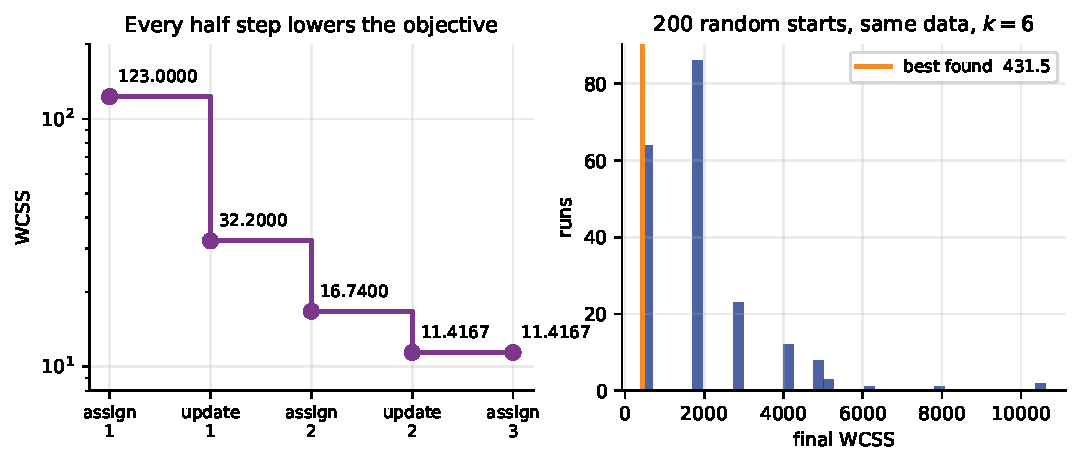
\includegraphics[width=0.92\textwidth]{wcss.pdf}
  \caption{Left: the objective after every half step of the hand run, on a
    log scale. Right: the final WCSS of $200$ single runs of $k$-means from
    uniformly random initial centroids on one fixed data set --- $106$
    distinct values.}
  \label{fig:wcss}
\end{figure}

\subsection{But only to a local optimum}
\label{sec:local}

The termination argument said nothing about optimality, and it could not
have: $k$-means is NP-hard and Lloyd's algorithm is four lines long.

Here is the demonstration. Six well-separated Gaussian blobs, $600$ points,
$k = 6$, twenty runs that differ only in the random seed used to place the
initial centroids.

\begin{lstlisting}
X, y = make_blobs(n_samples=600, centers=6, cluster_std=0.62, random_state=7)
for s in range(20):
    km = KMeans(n_clusters=6, init="random", n_init=1, random_state=s).fit(X)
    print(s, km.inertia_, adjusted_rand_score(y, km.labels_), km.n_iter_)
\end{lstlisting}
\begin{codeout}
  seed     inertia      ARI   n_iter        seed     inertia      ARI   n_iter
     0    431.5370   1.0000      3            10   1720.3550   0.7697      5
     1    431.5370   1.0000      2            11    431.5370   1.0000      3
     2    431.5370   1.0000      5            12   1883.8297   0.7673      7
     3   2740.4734   0.7787      5            13    431.5370   1.0000      5
     4   1720.5136   0.7693      7            14   1719.5194   0.7697      6
     5    431.5370   1.0000      5            15   2737.9794   0.7718      6
     6   2737.2417   0.7713      6            16    431.5370   1.0000      3
     7   5010.5833   0.5825      5            17   1719.5313   0.7697      6
     8   1884.4493   0.7673      9            18    431.5370   1.0000      5
     9   1885.0220   0.7677      6            19    431.5370   1.0000      3
distinct final WCSS values reached: 12
best  431.5370      worst 5010.5833      worst/best = 11.6110
\end{codeout}

Twelve distinct answers from twenty runs. Nine of them recover the blobs
exactly (ARI $1.000$); ten land near ARI $0.77$; one gets $0.58$. Every one of
those twelve is a genuine local optimum: no single point can be reassigned and
no centre moved to improve it. The algorithm did not fail. It converged. It
just converged somewhere else.

The failure always has the same shape, and Figure~\ref{fig:seeds} shows it:
two initial centres land inside the same true blob, so that blob is split in
two, and two other true blobs are consequently merged. Nothing can repair it,
because moving one centre across the empty space between blobs makes the
objective worse before it makes it better --- and Lloyd's algorithm only ever
goes downhill.

\begin{figure}[htbp]
  \centering
  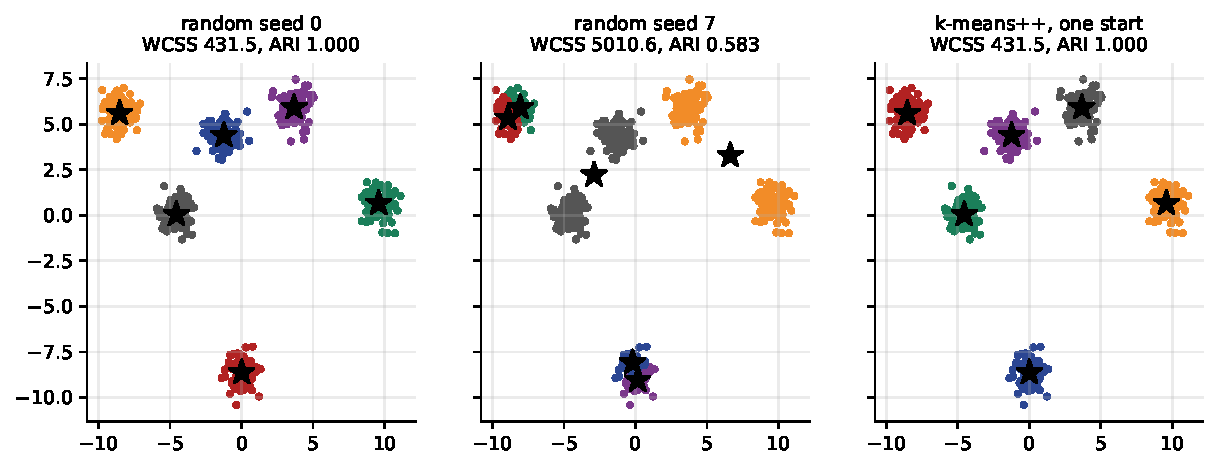
\includegraphics[width=0.92\textwidth]{seeds.pdf}
  \caption{Three runs on the same $600$ points. Left: a good random seed.
    Middle: a bad one --- notice the two centroids inside the lower-left blob
    and the three true blobs fused on the right. Right: one
    $k$-means\texttt{++} start, no restarts.}
  \label{fig:seeds}
\end{figure}

\subsection{$k$-means\texttt{++} and \texttt{n\_init}}

There are two independent fixes, and you should normally use both.

\textbf{Restart.} Run the whole algorithm several times from different random
starts and keep the run with the lowest \texttt{inertia\_}. This is what
\texttt{n\_init} does. It costs \texttt{n\_init} times as much, and since a
$k$-means fit on $600$ points takes a millisecond, that is the cheapest
insurance available.

\textbf{Seed better.} $k$-means\texttt{++} (Arthur and Vassilvitskii, 2007)
chooses the first centre uniformly at random and then each subsequent centre
with probability proportional to $D(x)^2$, the squared distance from $x$ to
the nearest centre already chosen. Points far from everything chosen so far
are overwhelmingly likely to be picked, so the initial centres spread out.
The paper proves
$\mathbb{E}[\phi] \le 8(\ln k + 2)\,\phi_{\text{OPT}}$ --- a genuine
approximation guarantee, before Lloyd's algorithm has run at all.

\begin{lstlisting}
for init in ("random", "k-means++"):
    ins = [KMeans(n_clusters=6, init=init, n_init=1,
                  random_state=s).fit(X).inertia_ for s in range(200)]
    print(init, np.mean(ins), min(ins), max(ins))
\end{lstlisting}
\begin{codeout}
  init         mean WCSS    best      worst   % reaching best
  random      1907.6245  431.5370 10621.5284      32.0
  k-means++    437.9858  431.5370  1721.3003      99.5

  n_init =  1 (random)   : mean 1836.8521   worst 10621.5284   % at best  35.0
  n_init =  3 (random)   : mean  948.5171   worst  2737.7477   % at best  62.5
  n_init = 10 (random)   : mean  463.7369   worst  1719.5313   % at best  97.5
  n_init = 25 (random)   : mean  431.5370   worst   431.5370   % at best 100.0
  n_init =  1 (k-means++): mean  431.5370   worst   431.5370   % at best 100.0
  n_init =  3 (k-means++): mean  431.5370   worst   431.5370   % at best 100.0
\end{codeout}

Read the two columns together. A single uniformly random start reaches the
best solution $32\%$ of the time; a single $k$-means\texttt{++} start reaches
it $99.5\%$ of the time. Ten random restarts get to $97.5\%$ --- roughly what
one careful seeding achieves on its own.

\begin{codeout}
  n_init =  1  0.0009 s   (exactly  1x the starts of n_init=1)
  n_init = 10  0.0059 s   (exactly 10x the starts of n_init=1)
  n_init = 50  0.0227 s   (exactly 50x the starts of n_init=1)
\end{codeout}

\begin{caution}[Timings are the one thing a seed cannot fix]
Every other number in these notes reproduces exactly. \textbf{The seconds do
not.} They depend on your processor, your BLAS build and what else is running,
and repeated runs of the identical code on the same machine moved the
PAM-against-$k$-means ratio of Section~\ref{sec:medoid} between $98\times$ and
$150\times$.

So the seconds are reported as a measurement and never as a property. Where
this lecture makes a cost claim it also gives the count behind it --- $m$
restarts is exactly $m$ times the work of one; PAM needs $n(n-1)/2$ distances
before its first swap against $k$-means' $nk$ per iteration --- and those are
the same on every machine. If your seconds differ from mine, you are right.
\end{caution}

\begin{caution}[Know what your defaults are]
scikit-learn's \texttt{n\_init} default is \texttt{"auto"}, which resolves to
\textbf{1} when \texttt{init="k-means++"} and \textbf{10} when
\texttt{init="random"}. That is a sensible pair of choices --- but if you set
\texttt{init="random"} and \texttt{n\_init=1} because a tutorial told you to,
you have opted into the $32\%$ row of the table above. \textbf{Never report a
$k$-means result from a single random start}, and always record
\texttt{random\_state}.
\end{caution}

\begin{tryit}
Take the six-blob data above, run \texttt{KMeans} with
\texttt{init="random", n\_init=1} for seeds $0$ to $19$, and print
\texttt{km.inertia\_}. You should see exactly two values dominate: $431.5370$
(nine times) and something near $1720$ or $2737$. Then plot the run with seed
$7$ and count the centroids inside each visible blob.
\end{tryit}

% =========================================================================
\section{Choosing $k$}
\label{sec:k}

\subsection{Why the objective cannot choose for you}

WCSS falls monotonically as $k$ increases, and reaches exactly zero at
$k = n$. So you cannot pick $k$ by minimising the objective; you would always
get $k = n$. Two heuristics are in universal use, and neither of them is a
criterion.

\textbf{The elbow.} Plot WCSS against $k$ and look for the point where the
\emph{rate} of improvement collapses --- where adding another cluster stops
buying much. There are at least two reasonable ways to automate this, and
Section~\ref{sec:k} below shows them disagreeing with each other.

\textbf{The silhouette.} For each point $i$, let $a(i)$ be its mean distance
to the other members of its own cluster and $b(i)$ its mean distance to the
members of the nearest \emph{other} cluster. Then
\begin{equation}
  s(i) = \frac{b(i) - a(i)}{\max\bigl(a(i),\ b(i)\bigr)} \in [-1, 1],
  \label{eq:sil}
\end{equation}
and the silhouette score is the average of $s(i)$ over all points. Unlike
WCSS it does not fall automatically with $k$, so it \emph{can} be maximised
--- which makes it feel like a criterion. It is not. It rewards compact,
well-separated, roughly spherical clusters, which is to say it rewards
exactly the shape $k$-means is looking for. On the two moons of
Section~\ref{sec:assume}, the silhouette prefers the wrong answer.

\subsection{A case where they agree, and a case where they do not}

\begin{lstlisting}
X, y = make_blobs(n_samples=500, centers=4, cluster_std=0.70, random_state=11)
for k in range(1, 11):
    km = KMeans(n_clusters=k, n_init=10, random_state=0).fit(X)
    print(k, km.inertia_,
          silhouette_score(X, km.labels_) if k > 1 else None)
\end{lstlisting}
\begin{codeout}
   k      WCSS     drop   silhouette
   1   20345.30       --   --
   2    8095.80 12249.50   0.5960
   3    1880.33  6215.47   0.7668
   4     493.25  1387.08   0.7973
   5     442.57    50.68   0.7008
   6     397.59    44.98   0.5702
   7     357.67    39.92   0.4359
   8     316.34    41.33   0.3287
\end{codeout}

On four clean blobs the drop column is unambiguous: $1387$ at $k=4$ and then
$50.7$ at $k=5$, a collapse by a factor of $27$. The silhouette peaks at
$k=4$. Everything agrees, and the truth is $4$.

Now iris, standardised:

\begin{codeout}
   k      WCSS   silhouette      ARI vs species
   1   600.0000   --       --
   2   222.3617   0.5818   0.5681
   3   139.8205   0.4599   0.6201
   4   114.0925   0.3869   0.4728
   5    90.8076   0.3455   0.4205
   6    80.0225   0.3257   0.3563
   7    71.6126   0.3323   0.4088
   8    62.8661   0.3449   0.3136
\end{codeout}

The silhouette peaks at $k = 2$, at $0.5818$. The ARI against the true
species peaks at $k = 3$, at $0.6201$. And the elbow depends on how you
automate it:

\begin{lstlisting}
def chord(W, kmax=8):                     # the "kneedle" rule
    ks = np.arange(1, kmax+1)
    x = (ks - 1) / (kmax - 1)
    w = np.array([W[k] for k in ks]); z = (w - w[-1]) / (w[0] - w[-1])
    return int(ks[np.argmax(np.abs(z + x - 1) / np.sqrt(2))])

def ratio(W, kmax=8):                     # largest collapse in the drops
    drop = {k: W[k-1] - W[k] for k in range(2, kmax+1)}
    return max({k: drop[k]/drop[k+1] for k in range(2, kmax)}.items(),
               key=lambda t: t[1])[0]
\end{lstlisting}
\begin{codeout}
  four clean blobs   chord rule k = 3   drop-ratio rule k = 4
      drop ratios       {2: 1.97, 3: 4.48, 4: 27.37, 5: 1.13, 6: 1.13, 7: 0.97}
  iris               chord rule k = 3   drop-ratio rule k = 2
      drop ratios       {2: 4.58, 3: 3.21, 4: 1.1, 5: 2.16, 6: 1.28, 7: 0.96}

  summary            chord  ratio  silhouette  ARI-best  truth
  four clean blobs       3      4           4         4      4
  iris                   3      2           2         3      3
\end{codeout}

\begin{keyidea}
On iris, two automations of the \emph{same} heuristic disagree with each
other before the silhouette is even consulted. ``Use the elbow method'' is not
a procedure; it is an invitation to look at a graph.
\end{keyidea}

\begin{figure}[htbp]
  \centering
  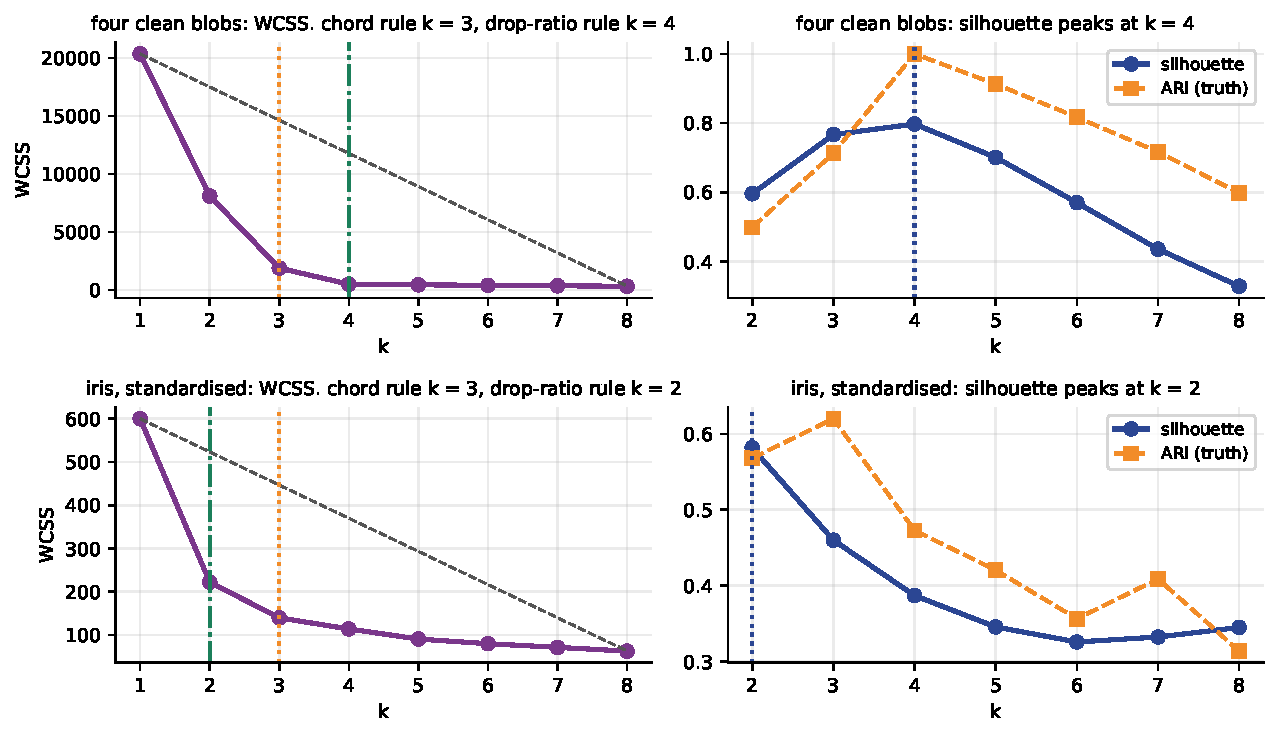
\includegraphics[width=0.98\textwidth]{choosek.pdf}
  \caption{Left column: WCSS with the end-to-end chord (dashed grey) and the
    two elbow verdicts marked. Right column: silhouette against ARI with the
    true labels. Top row, four clean blobs; bottom row, iris.}
  \label{fig:choosek}
\end{figure}

It is worth being clear about \emph{why} iris behaves like this rather than
treating it as a defect. Two of the three iris species genuinely overlap in
these four measurements. The data really does look like two clusters. The
unsupervised criteria are describing the data correctly; it is the assumption
that ``number of clusters'' equals ``number of classes in the label column''
that is wrong. Those are different quantities, and on real data they usually
differ.

\subsection{The most important warning in this section}

$k$-means always returns $k$ clusters. It has no way of returning ``there is
no structure here''. Here are $500$ points drawn uniformly at random in the
unit square:

\begin{codeout}
   k      WCSS   silhouette
   1    80.6344   --
   2    49.7154   0.3592
   3    31.2614   0.3839
   4    20.3558   0.4060
   5    16.6794   0.3853
   6    13.7743   0.3917
   7    11.3759   0.3895
\end{codeout}

The curve is smooth --- there is no elbow, correctly --- but the silhouette
still has a maximum, at $k = 4$, with a value of $0.4060$ that is not
obviously smaller than what many real data sets produce. If you had run this
inside a pipeline that selects $k$ by maximising the silhouette, you would
have got four confident clusters out of pure noise.

\begin{caution}[Always look at the clustering, not only at the score]
Before you believe a $k$, check the cluster sizes (a $499/1$ split is outlier
peeling, not structure), project to two dimensions and look, and if you have
any labels at all, cross-tabulate. A number from a heuristic is a hypothesis,
not a result.
\end{caution}

% =========================================================================
\section{What $k$-means assumes, and where it breaks}
\label{sec:assume}

\subsection{Three assumptions, all in one formula}

Section~\ref{sec:part} pulled them out of equation~\eqref{eq:wcss} and they
are worth restating as three claims about your data that $k$-means is
implicitly making.

\textbf{Clusters are spherical (more precisely, convex).} A cluster is
represented by a single point and membership is decided by nearest
centroid, so the clusters are Voronoi cells. Nothing $k$-means returns can
have a concave boundary.

\textbf{Clusters are of similar size.} The sum in \eqref{eq:wcss} runs over
points. A cluster of $400$ contributes ten times as many terms as one of
$40$, so splitting the large one is often cheaper than respecting the small
one.

\textbf{Clusters have similar spread.} A tight cluster and a diffuse one at
the same distance from a centroid are treated identically; the criterion has
no notion of local density.

\begin{keyidea}
These are not bugs to be fixed with a parameter. They are the definition of
what $k$-means is looking for. If your clusters are not like that, $k$-means
will still return $k$ of them, and they will be wrong.
\end{keyidea}

\subsection{Four data sets it cannot handle}

\begin{lstlisting}
Xm, ym = make_moons(n_samples=400, noise=0.06, random_state=0)
Xc, yc = make_circles(n_samples=400, factor=0.45, noise=0.05, random_state=0)
Xu, yu = make_blobs(n_samples=[400, 40, 40],
                    centers=[[0,0], [7,0], [7,4]],
                    cluster_std=[1.9, 0.35, 0.35], random_state=3)
for nm, X, y, k in rows:
    km = KMeans(n_clusters=k, n_init=10, random_state=0).fit(X)
    print(nm, adjusted_rand_score(y, km.labels_), np.bincount(km.labels_))
\end{lstlisting}
\begin{codeout}
  data                    k     k-means ARI    sizes found
  two moons               2        0.274       195,205
  concentric circles      2       -0.002       207,193
  two long thin bands     2       -0.001       399,401
  very unequal sizes      3        0.288       208,176,96
  true sizes for the last row: 400,40,40
\end{codeout}

Look at the sizes column before the ARI column. Every answer is close to an
equal split, because that is what minimising a sum of squares over a convex
partition wants. On the last row the truth is $400/40/40$; $k$-means returns
$208/176/96$, which is to say it \textbf{cut the big cluster into three and
merged the two small ones into the pieces}. An ARI at or below zero, as on the
circles and the bands, means the answer is no better than a random partition
of the same shape.

The two long thin bands deserve a sentence of their own. They are two
horizontal strips at $y \approx 0$ and $y \approx 2.2$, each $20$ units long.
$k$-means returns a \emph{left} half and a \emph{right} half, sizes
$399/401$. It is not confused; it is right. Two long strips have enormous
within-strip variance, and two compact halves have less. The mismatch is
between the objective and the data, and there is no parameter to tune.

\begin{figure}[htbp]
  \centering
  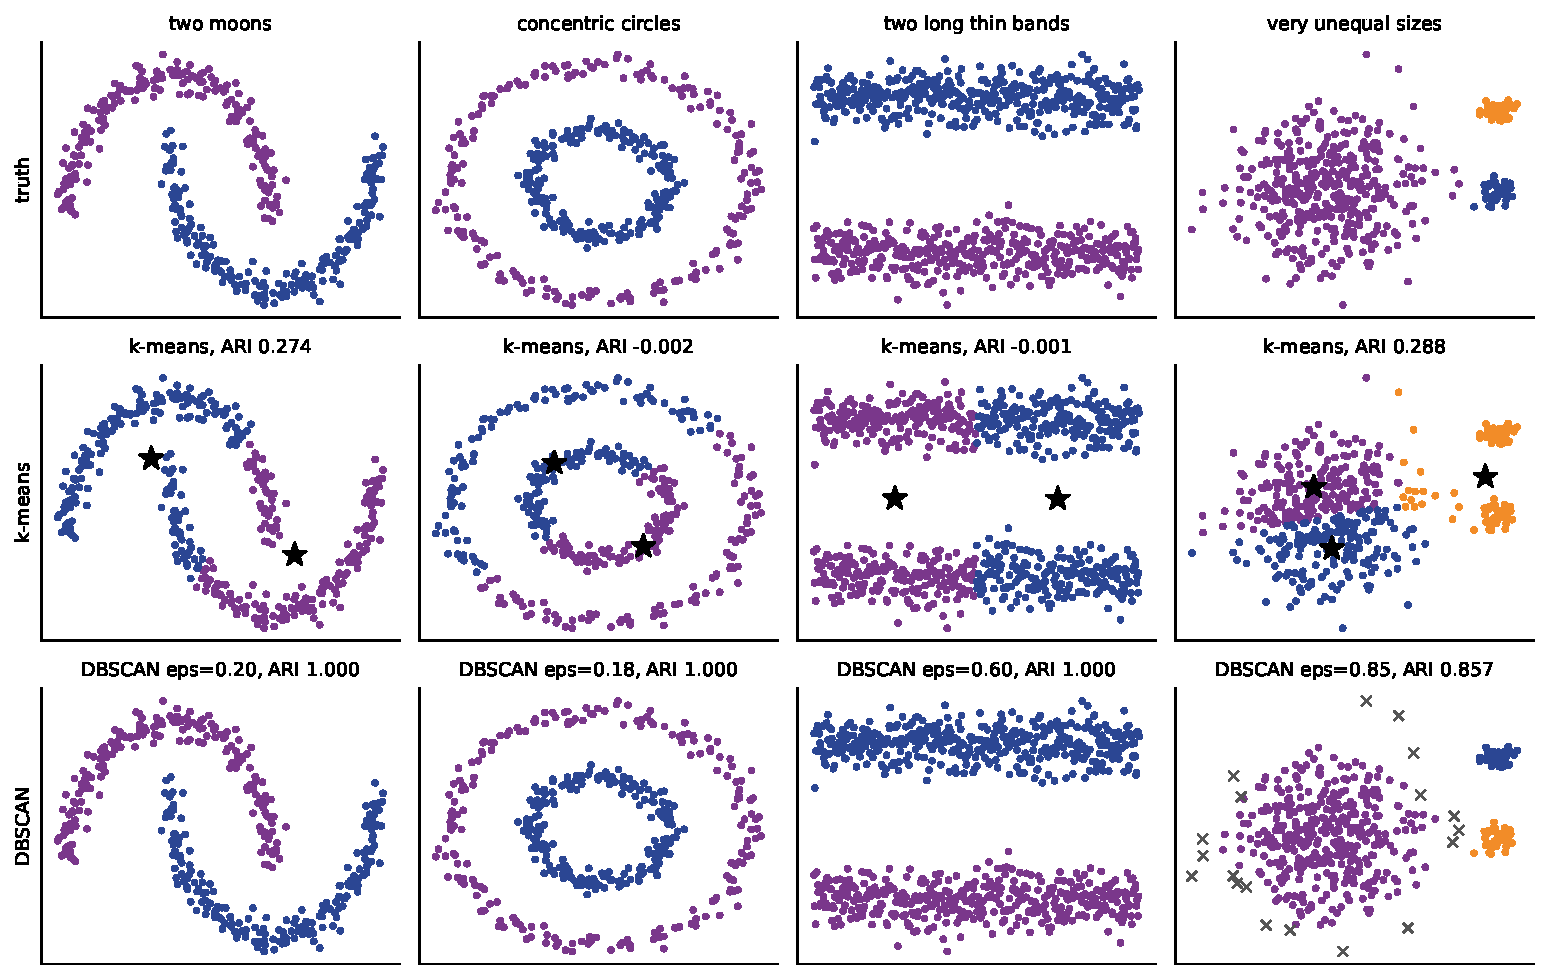
\includegraphics[width=0.84\textwidth]{assumptions.pdf}
  \caption{Four data sets. Top: the truth. Middle: $k$-means with the correct
    $k$, centroids starred. Bottom: DBSCAN, which we come to in
    Section~\ref{sec:dbscan}, scoring ARI $1.000$, $1.000$, $1.000$ and
    $0.857$ on the same four sets.}
  \label{fig:assumptions}
\end{figure}

\subsection{And the mean is not robust}

Take the same seven hand-worked points and add \textbf{one} extra point at
$(12, 9)$.

\begin{codeout}
  k-means  without the outlier: centres [[1.6667, 2.0], [7.0,  4.75]]  sizes [3, 4]
  k-means  with    the outlier: centres [[2.5,    2.5], [8.75, 6.0 ]]  sizes [4, 4]
  k-medoid without the outlier: medoids ['P1','P5'] at [[1,2],[7,5]]   E =  7.8929
  k-medoid with    the outlier: medoids ['P1','P5'] at [[1,2],[7,5]]   E = 14.2960
  the right-hand centre moved 2.1506; the right-hand medoid did not move at all.
\end{codeout}

One point did two things. It moved the right-hand centroid by $2.1506$ --- and
because the centroid moved, the \emph{partition} changed: $P_4$ was pulled out
of the right-hand cluster into the left one, giving $4/4$ instead of $3/4$. A
single observation, less than $13\%$ of the data, rewrote the answer.

The $k$-medoid answer (Section~\ref{sec:medoid} defines it properly) did not
move at all, because a medoid is an \emph{observation}. It cannot drift; it
can only jump to a different observation.

\begin{codeout}
  outlier at    k-means: right centre      shift   sizes   k-medoids: right medoid
  none         (  7.0000,  4.7500)        0.0000   3,4     P5   (7, 5)
  (8, 6.0)     (  7.2000,  5.0000)        0.3202   3,5     P5   (7, 5)
  (10, 7.5)    (  7.6000,  5.3000)        0.8139   3,5     P5   (7, 5)
  (12, 9.0)    (  8.7500,  6.0000)        2.1506   4,4     P5   (7, 5)
  (16, 12.0)   ( 16.0000, 12.0000)       11.5569   1,7     OUT  (16, 12)
  (20, 15.0)   ( 20.0000, 15.0000)       16.5548   1,7     OUT  (20, 15)
  (40, 30.0)   ( 40.0000, 30.0000)       41.5519   1,7     OUT  (40, 30)
\end{codeout}

Be honest about the last three rows. Beyond about $(16,12)$ the outlier is so
far away that spending an entire cluster on it is cheaper than any
alternative, and \emph{both} methods do exactly that: sizes $1/7$, all seven
real points fused into one cluster. $k$-medoids is more robust, not immune.

\begin{figure}[htbp]
  \centering
  
\includegraphics[width=0.90\textwidth]{outlier.pdf}
  \caption{The seven points with no outlier, with an outlier at $(12,9)$, and
    with one at $(16,12)$. Blue stars are $k$-means centroids, green squares
    are $k$-medoids. At $(12,9)$ the centroid has moved and the partition has
    changed; the medoids have not moved. At $(16,12)$ both methods give up a
    cluster to the outlier.}
  \label{fig:outlier}
\end{figure}

% =========================================================================
\section{$k$-medoids and PAM}
\label{sec:medoid}

\subsection{Change one word}

The $k$-medoids objective is
\begin{equation}
  E \;=\; \sum_{j=1}^{k}\ \sum_{x \in C_j} d\bigl(x,\ o_j\bigr),
  \label{eq:medoid}
\end{equation}
where each $o_j$ is an \textbf{object of the data set} --- the \emph{medoid}
of cluster $j$ --- and $d$ is \textbf{any} dissimilarity. Compare with
equation~\eqref{eq:wcss}: the representative is now a real observation rather
than a computed mean, the distance is not squared, and there is no requirement
that the data live in a vector space at all. This objective is often called
the \emph{absolute-error criterion} in the data-mining literature.

Three consequences follow, and each of them is a reason the method exists.

\textbf{The representative is interpretable.} ``The archetypal customer of
this segment is customer \#4417'' is a sentence you can act on. ``The
archetypal customer has $2.7$ children and lives $0.4$ of the way to Delhi''
is not.

\textbf{Any dissimilarity works.} Edit distance between strings, Jaccard
between sets, Gower for mixed types, or a precomputed matrix from a domain
expert. There is no mean of two DNA sequences; there is a medoid.

\textbf{It is far less sensitive to outliers.} An unsquared distance to a
fixed observation cannot be dragged the way a squared distance to a movable
mean can.

\begin{keyidea}
$k$-means asks ``where should the centre be?''. $k$-medoids asks ``which one
of you is the centre?''. Restricting the answer to a data point costs
computation and buys robustness, interpretability, and the freedom to use any
dissimilarity you like.
\end{keyidea}

\subsection{PAM: Partitioning Around Medoids}

The standard algorithm, due to Kaufman and Rousseeuw (1990), has two phases.

\begin{lstlisting}
BUILD : o_1 = the object minimising total dissimilarity to everything else
        repeat until k medoids: add the object that reduces E the most

SWAP  : repeat
            for every medoid o_i and every non-medoid o_h:
                compute dE, the change in E if o_i were replaced by o_h
            if the best dE < 0: perform that swap
            else: stop
\end{lstlisting}

Here is a complete implementation. It is short because the SWAP evaluation can
be vectorised: for a fixed medoid $o_i$ to be removed, define
$\text{base}[x]$ as $x$'s distance to its nearest \emph{remaining} medoid;
then the cost after inserting candidate $o_h$ is
$\sum_x \min(\text{base}[x],\ d(x,o_h))$, which is a single reduction over the
whole distance matrix.

\begin{lstlisting}
def pam_cost(D, med):
    return float(D[:, med].min(axis=1).sum())

def pam_swap(D, med):
    n, med = D.shape[0], list(med)
    while True:
        S  = np.sort(D[:, med], axis=1)
        d1, d2 = S[:, 0], S[:, 1]
        a1 = np.array(med)[np.argmin(D[:, med], axis=1)]
        best, bswap = float(d1.sum()), None
        for i in med:
            base = np.where(a1 == i, d2, d1)
            cand = np.minimum(base[:, None], D).sum(axis=0)
            cand[med] = np.inf
            h = int(np.argmin(cand))
            if cand[h] < best - 1e-12:
                best, bswap = float(cand[h]), (i, h)
        if bswap is None:
            return sorted(med), pam_cost(D, med)
        med[med.index(bswap[0])] = bswap[1]
\end{lstlisting}

That inner loop does one $n \times n$ reduction per medoid, so one SWAP
iteration costs $O(k n^2)$ --- which is Han, Kamber and Pei's
$O\bigl(k(n-k)^2\bigr)$ per iteration. A textbook triple loop has the same
order with a constant a few hundred times worse. Note also that PAM works
from the dissimilarity matrix, so it needs $O(n^2)$ \emph{memory}, exactly
like hierarchical clustering.

\subsection{By hand: all twenty-one medoid pairs}

On the seven points of Section~\ref{sec:hand} with $k = 2$ there are only
$\binom{7}{2} = 21$ candidate medoid pairs, so we can score every one. First
the proximity matrix:

\begin{codeout}
              P1      P2      P3      P4      P5      P6      P7
  P1      0.0000  1.4142  1.4142  4.4721  6.7082  7.2801  8.0623
  P2      1.4142  0.0000  2.0000  4.2426  6.4031  6.7082  7.8102
  P3      1.4142  2.0000  0.0000  3.1623  5.3852  6.0828  6.7082
  P4      4.4721  4.2426  3.1623  0.0000  2.2361  3.0000  3.6056
  P5      6.7082  6.4031  5.3852  2.2361  0.0000  1.4142  1.4142
  P6      7.2801  6.7082  6.0828  3.0000  1.4142  0.0000  2.0000
  P7      8.0623  7.8102  6.7082  3.6056  1.4142  2.0000  0.0000
\end{codeout}

\begin{worked}[Scoring the pair $\{P_1, P_5\}$]
Each point contributes its distance to whichever of the two medoids is
nearer:
\[
\begin{array}{lccc}
  & d(\cdot, P_1) & d(\cdot, P_5) & \min\\[2pt]
  P_1 & 0.0000 & 6.7082 & 0.0000\\
  P_2 & 1.4142 & 6.4031 & 1.4142\\
  P_3 & 1.4142 & 5.3852 & 1.4142\\
  P_4 & 4.4721 & 2.2361 & 2.2361\\
  P_5 & 6.7082 & 0.0000 & 0.0000\\
  P_6 & 7.2801 & 1.4142 & 1.4142\\
  P_7 & 8.0623 & 1.4142 & 1.4142
\end{array}
\]
$E = 0 + 1.4142 + 1.4142 + 2.2361 + 0 + 1.4142 + 1.4142 = \mathbf{7.8929}$.
Note there is no squaring anywhere.
\end{worked}

All twenty-one:

\begin{codeout}
  {P1,P2}  E =  26.5784      {P3,P4}  E =  12.2558
  {P1,P3}  E =  22.7526      {P3,P5}  E =   8.4787
  {P1,P4}  E =  11.6700      {P3,P6}  E =   9.8284
  {P1,P5}  E =   7.8929  <-- best     {P3,P7}  E =   9.9907
  {P1,P6}  E =   9.2426      {P4,P5}  E =  14.7055
  {P1,P7}  E =   9.8482      {P4,P6}  E =  15.2913
  {P2,P3}  E =  22.7526      {P4,P7}  E =  15.2913
  {P2,P4}  E =  12.2558      {P5,P6}  E =  22.1468
  {P2,P5}  E =   8.4787      {P5,P7}  E =  22.1468
  {P2,P6}  E =   9.8284      {P6,P7}  E =  24.4853
  {P2,P7}  E =  10.4340
  best medoid pair: {P1, P5}   E = 7.8929
\end{codeout}

Twenty-one is small enough to brute-force. At $n = 100$ with $k = 5$ it is
$\binom{100}{5} = 75{,}287{,}520$, which is why PAM does a local search.

\subsection{By hand: the SWAP step}

Start deliberately badly, with both medoids in the left-hand clump:

\begin{codeout}
  start with medoids {P1, P2}, E = 26.5784
  step 1: best swap  P2 -> P5   dE = -18.6855   E =  7.8929
  step 2: best swap  P1 -> P2   dE =  +0.5858   E =  8.4787
          no swap improves E -- STOP
  final medoids: {P1, P5}   E = 7.8929
\end{codeout}

Read step 2 carefully, because it is the stopping condition. Ten candidate
swaps remain, and the \emph{best} of them still makes $E$ worse, by $0.5858$.
Since no single swap improves the objective, PAM stops --- at a local optimum
of the swap neighbourhood, by exactly the same kind of argument as $k$-means:
$E$ never increases, there are $\binom{n}{k}$ medoid sets, so the loop
terminates.

\begin{caution}[PAM is a hill-climber too]
It is tempting to think that because $k$-medoids does not involve random
initialisation in its BUILD phase, it gives ``the'' answer. It gives a
\emph{deterministic} answer, which is not the same as an optimal one. PAM
from the BUILD phase and PAM from $\{P_1,P_2\}$ agree here, but that is a
property of seven clean points.
\end{caution}

\subsection{Robustness, measured}

Two clean blobs of $150$ points at $(0,0)$ and $(6,0)$, standard deviation
$0.7$. Add a handful of points scattered uniformly in $[20,45]^2$. The
``centre error'' below is the largest distance from a true centre to the
nearest thing the method returned; the ARI is computed on the $300$ genuine
points only, so it answers ``did the contamination break the real clusters?''.

\begin{codeout}
  outliers  k-means: centre error  ARI  |  k-medoids: medoid error  ARI
       0              0.0951   1.000  |                0.0905   1.000
       2              0.5210   1.000  |                0.0905   1.000
       5              3.0826   0.000  |                0.0905   1.000
      10              3.0826   0.000  |                0.0905   1.000
      20              3.0826   0.000  |                4.0563   0.000
\end{codeout}

\textbf{Five} outliers out of $305$ points destroy $k$-means completely. With
$k = 2$ it spends one centre on the little clump of outliers and one on
everything else, so the two real clusters are merged into one and the ARI
falls from $1.000$ to $0.000$. Two outliers are already enough to drag a
centre five times further off ($0.0951 \to 0.5210$) without yet breaking the
partition --- the damage is continuous, and it starts immediately.
$k$-medoids does not move at all until there are twenty, at which point the
outliers are numerous enough to be a genuine cluster and arguably it is right
to give them one.

\subsection{Where $k$-means cannot go at all}

Eight English words, Levenshtein edit distance, $k=2$. There is no arithmetic
mean of two words, so $k$-means is not merely worse here: it is undefined.

\begin{lstlisting}
words = ["cluster","clusters","clustered","medoid","medoids",
         "density","densities","dense"]
Dw = np.array([[lev(a, b) for b in words] for a in words], float)
med, cost = pam_swap(Dw, pam_build(Dw, 2))
print([words[i] for i in med], cost)
\end{lstlisting}
\begin{codeout}
edit-distance matrix over 8 words; PAM with k = 2
  medoids: ['cluster', 'density']   E = 19.0
  cluster 1: cluster, clusters, clustered
  cluster 2: medoid, medoids, density, densities, dense
\end{codeout}

\subsection{What it costs}

\begin{codeout}
     n    k   PAM time (s)   k-means time (s)    ratio
   250    4        0.0016            0.0037           0.4x
   500    4        0.0100            0.0049           2.1x
  1000    4        0.0378            0.0054           7.0x
  2000    4        0.1817            0.0066          27.6x
  4000    4        1.1032            0.0073         150.3x
  fitted exponent for PAM,  t = c n^p :  p = 2.30

       n      PAM: n(n-1)/2 k-means: n*k per it.        ratio
    4000          7,998,000               16,000       499.9x
\end{codeout}

At $n = 250$, PAM is faster than $k$-means with ten restarts. At $n = 4000$ it
is two orders of magnitude slower, and the fitted growth exponent is about
$2.3$ against $k$-means' near-linear behaviour.

Those seconds are a measurement on one machine and the ratio moved between
$98\times$ and $150\times$ on repeated runs of the same code, so take the
exact version from the last two lines of that block: before PAM can evaluate a
single swap it needs the whole distance matrix, $n(n-1)/2 = 7{,}998{,}000$
distances at $n = 4000$, while $k$-means computes $nk = 16{,}000$ per Lloyd
iteration. A factor of $\mathbf{500}$, on any machine.

Extrapolate: at $n = 100{,}000$ one SWAP
iteration considers $k(n-k)^2 = 5 \times 99995^2 \approx 5.0 \times 10^{10}$
candidate evaluations, and the $n \times n$ float64 matrix it needs is
$74.5$\,GiB.

\begin{codeout}
     n     k   k(n-k)^2 per SWAP iteration   n x n float64 matrix
      100   5                      45125              0.1 MiB
     1000   5                4.95012e+06              7.6 MiB
    10000   5                  4.995e+08            762.9 MiB
   100000   5                 4.9995e+10             74.5 GiB
\end{codeout}

That table is the entire motivation for the next section.

% =========================================================================
\section{CLARA: Clustering Large Applications}
\label{sec:clara}

\subsection{The idea}

If PAM is infeasible at $n = 100{,}000$ and the cost is driven by $n$, then
reduce $n$. CLARA (Kaufman and Rousseeuw, 1990) draws a random sample, runs
PAM on the sample, and then uses the resulting medoids to classify
\emph{all} $n$ objects. It repeats this a few times and keeps whichever set of
medoids gives the lowest total cost over the whole data set.

\begin{lstlisting}
def clara(X, k, nsamp=5, size=None, seed=0):
    rng, n = np.random.default_rng(seed), len(X)
    size = size or min(n, 40 + 2 * k)          # Kaufman & Rousseeuw's rule
    best = None
    for _ in range(nsamp):
        idx = rng.choice(n, size=size, replace=False)
        Ds  = squareform(pdist(X[idx]))
        m, _ = pam_swap(Ds, pam_build(Ds, k))
        med  = idx[m]                                  # back to global ids
        cost = float(cdist(X, X[med]).min(axis=1).sum())   # ALL n objects
        if best is None or cost < best[1]:
            best = (med, cost)
    med, cost = best
    return med, np.argmin(cdist(X, X[med]), axis=1), cost
\end{lstlisting}

Two details make this work and are worth naming.

\textbf{The evaluation uses all $n$ objects.} If CLARA scored each candidate
medoid set on its own sample, a lucky sample would look better than it is.
Scoring on the full data set removes that bias at a cost of $O(k(n-k))$ per
sample, which is linear.

\textbf{The dissimilarity matrix is $s \times s$, not $n \times n$.} With
$s = 40 + 2k$, that is a matrix of about fifty rows. The whole reason PAM was
unavailable has been removed.

The complexity is $O\bigl(k s^2 + k(n-k)\bigr)$ per sample --- quadratic in
the \emph{sample} size and linear in $n$.

\subsection{Measured against PAM}

\begin{codeout}
      n    PAM time   PAM cost    CLARA time  CLARA cost   cost ratio   speed-up
    500       0.011    661.537       0.002    707.320      1.0692        5.0x
   1000       0.034   1290.963       0.003   1342.576      1.0400       10.5x
   2000       0.259   2636.569       0.003   2842.923      1.0783       89.0x
   4000       1.731   5261.167       0.004   5490.189      1.0435      421.0x
\end{codeout}

CLARA's time barely changes with $n$, because the PAM it runs is always on
fifty objects; only the final assignment sweep grows. \textbf{The cost ratio
is the reproducible column}: consistently within $4$--$8\%$ of PAM's, the
same on every machine, because it is arithmetic on the data and not a
measurement. The speed-up column is a timing and moved between $420\times$
and $520\times$ on repeated runs of the same code.

Say the speed claim exactly instead. One SWAP iteration of PAM at $n = 4000$,
$k = 5$ considers $k(n-k)^2 = 79{,}800{,}125$ candidate evaluations; CLARA
runs PAM on five samples of fifty, which is $5 \times k(s-k)^2 = 50{,}625$.
That is a factor of $\mathbf{1576}$, and it does not depend on your
processor.

\begin{figure}[htbp]
  \centering
  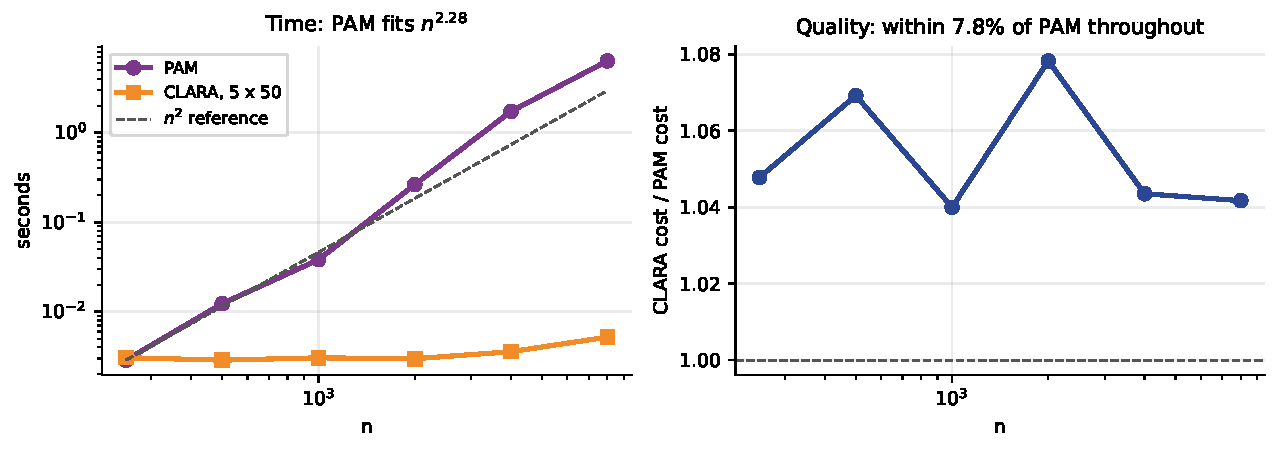
\includegraphics[width=0.90\textwidth]{clara.pdf}
  \caption{Left: run time on log-log axes, with an $n^2$ reference line. PAM
    fits $n^{2.15}$ over this range; CLARA is essentially flat. Right: CLARA's
    cost as a multiple of PAM's, never worse than about $7\%$.}
  \label{fig:clara}
\end{figure}

\subsection{Buying quality with sample size, and the price of randomness}

\begin{codeout}
  n = 4000, k = 5.  PAM reference: cost 5261.167   ARI 0.8404
  sample size   samples   CLARA cost   cost/PAM     ARI    time (s)
           20         5     5915.642     1.1244  0.8008     0.003
           50         5     5490.189     1.0435  0.8266     0.004
          100         5     5478.582     1.0413  0.8340     0.006
          250         5     5319.240     1.0110  0.8384     0.015
          500         5     5302.009     1.0078  0.8302     0.048
\end{codeout}

A sample of $20$ costs $12\%$ more than PAM. A sample of $500$ costs $0.8\%$
more and is still an order of magnitude faster than PAM at this $n$. The
sample size is the dial.

\begin{caution}[CLARA gives a different answer every time]
PAM is deterministic. CLARA is not: it depends on which objects were sampled.
\begin{codeout}
  seed   CLARA cost   cost/PAM     ARI
     0     5490.189     1.0435  0.8266
     1     5421.410     1.0305  0.8206
     3     5515.536     1.0483  0.8052
     5     5708.138     1.0850  0.8073
     7     5700.247     1.0835  0.8232
  CLARA over 10 seeds: cost 5421.410 to 5708.138 (spread 5.3%),
                       ARI 0.8052 to 0.8290
\end{codeout}
Report the seed, or increase \texttt{nsamp}, which is CLARA already doing the
restart trick internally.
\end{caution}

\subsection{One thing CLARA is not guilty of}

The usual criticism of CLARA is that a small cluster may never appear in any
sample, so its medoid can never be chosen. The arithmetic is real: in a data
set of $6040$ points with a cluster of $40$, a sample of $50$ contains
$50 \times 40/6040 = 0.331$ of them on average. But the conclusion does not
follow, and it is worth checking rather than repeating.

\begin{codeout}
  6040 points: two clusters of 3000 and one of 40
  expected number of the 40 in a sample of size 50: 0.331
  PAM   medoids at [[9.44, 0.43], [10.62, -0.51], [0.04, 0.02]]
        cost 7239.719   ARI 0.7457
  cost if a medoid is forced onto each true centre: 7502.069
  CLARA sample   50  cost 7269.834  ratio 1.0042  ARI 0.7426
  CLARA sample  200  cost 7263.726  ratio 1.0033  ARI 0.7503
  CLARA sample 1000  cost 7254.729  ratio 1.0021  ARI 0.7457
\end{codeout}

\textbf{PAM itself does not put a medoid on the small cluster.} It puts two
medoids inside one of the big ones. And the ``correct'' solution --- one
medoid at each true centre --- genuinely costs more: $7502$ against $7240$.
So this is a property of the \textbf{objective}, not of the sampling.
Minimising total dissimilarity does not reward small clusters; forty points
at distance $12$ contribute less than a slightly better split of three
thousand points. CLARA inherits the problem; it does not create it.

\begin{keyidea}
When a method gives an answer you dislike, check whether the objective
prefers your answer before blaming the algorithm. Here it does not, and the
right response is to change the objective (or the method) rather than the
implementation.
\end{keyidea}

% =========================================================================
\section{DBSCAN: density-based clustering}
\label{sec:dbscan}

\subsection{A different definition of ``cluster''}

Everything so far has said: a cluster is the set of objects nearest to a
representative. That single sentence forces convex clusters, forces you to
supply $k$, and forces every object into some cluster.

Density-based clustering says something else entirely: \textbf{a cluster is a
connected region in which the points are packed closely together, separated
from other such regions by sparser space}. Nothing in that definition mentions
shape, or $k$, and it leaves room for points that are in no dense region at
all. DBSCAN --- Density-Based Spatial Clustering of Applications with Noise,
Ester, Kriegel, Sander and Xu, KDD 1996 --- makes it precise.

\subsection{The definitions}

Two parameters: a radius $\varepsilon$ (\texttt{eps}) and a count
\emph{minPts} (\texttt{min\_samples}). The \textbf{$\varepsilon$-neighbourhood}
of a point $p$ is
\[
  N_\varepsilon(p) = \{q \in D : d(p,q) \le \varepsilon\},
\]
and in scikit-learn's convention it \textbf{includes $p$ itself}.

\begin{itemize}[leftmargin=*]
  \item $p$ is a \textbf{core point} if $|N_\varepsilon(p)| \ge$ minPts.
  \item $p$ is a \textbf{border point} if it is not core but lies in
    $N_\varepsilon(q)$ for some \emph{core} point $q$.
  \item $p$ is \textbf{noise} if it is neither. scikit-learn reports noise as
    label $-1$.
\end{itemize}

The relations that glue a cluster together:

\begin{itemize}[leftmargin=*]
  \item $q$ is \textbf{directly density-reachable} from $p$ if $p$ is core
    and $q \in N_\varepsilon(p)$.
  \item $q$ is \textbf{density-reachable} from $p$ if there is a chain
    $p = p_1, p_2, \ldots, p_m = q$ with each $p_{i+1}$ directly
    density-reachable from $p_i$ --- so all of $p_1, \ldots, p_{m-1}$ are
    core. This relation is transitive but \emph{not} symmetric: a border
    point is density-reachable from a core point but not the other way round.
  \item $p$ and $q$ are \textbf{density-connected} if both are
    density-reachable from some common core point $o$. This relation
    \emph{is} symmetric.
  \item A \textbf{cluster} is a maximal set of density-connected points.
    \textbf{Noise} is everything in no cluster.
\end{itemize}

\begin{keyidea}
Core points define the clusters; border points are attached to them; noise is
what is left. Because the clusters are grown by chaining short steps between
core points, they can be any shape at all --- and because nothing forces a
point into a cluster, DBSCAN can report that a point belongs to nothing.
\end{keyidea}

\subsection{Eleven points, by hand}

\begin{center}
\begin{tabular}{lccccccccccc}
  \toprule
  & $Q_1$ & $Q_2$ & $Q_3$ & $Q_4$ & $Q_5$ & $Q_6$ & $Q_7$ & $Q_8$ & $Q_9$
  & $Q_{10}$ & $Q_{11}$ \\
  \midrule
  $x$ & 1 & 2 & 1 & 2 & 3 & 7 & 8 & 8 & 9 & 5 & 11 \\
  $y$ & 1 & 1 & 2 & 2 & 3 & 3 & 3 & 4 & 5 & 6 & 1 \\
  \bottomrule
\end{tabular}
\end{center}

Take $\varepsilon = 1.5$ and minPts $= 3$. The distance matrix:

\begin{codeout}
          Q1     Q2     Q3     Q4     Q5     Q6     Q7     Q8     Q9    Q10    Q11
  Q1   0.000  1.000  1.000  1.414  2.828  6.325  7.280  7.616  8.944  6.403 10.000
  Q2   1.000  0.000  1.414  1.000  2.236  5.385  6.325  6.708  8.062  5.831  9.000
  Q3   1.000  1.414  0.000  1.000  2.236  6.083  7.071  7.280  8.544  5.657 10.050
  Q4   1.414  1.000  1.000  0.000  1.414  5.099  6.083  6.325  7.616  5.000  9.055
  Q5   2.828  2.236  2.236  1.414  0.000  4.000  5.000  5.099  6.325  3.606  8.246
  Q6   6.325  5.385  6.083  5.099  4.000  0.000  1.000  1.414  2.828  3.606  4.472
  Q7   7.280  6.325  7.071  6.083  5.000  1.000  0.000  1.000  2.236  4.243  3.606
  Q8   7.616  6.708  7.280  6.325  5.099  1.414  1.000  0.000  1.414  3.606  4.243
  Q9   8.944  8.062  8.544  7.616  6.325  2.828  2.236  1.414  0.000  4.123  4.472
  Q10  6.403  5.831  5.657  5.000  3.606  3.606  4.243  3.606  4.123  0.000  7.810
  Q11 10.000  9.000 10.050  9.055  8.246  4.472  3.606  4.243  4.472  7.810  0.000
\end{codeout}

Only two values in that table are inside $\varepsilon = 1.5$: $1.000$ (a
horizontal or vertical grid step) and $1.414 = \sqrt{2}$ (a diagonal step).
Everything from $2.000$ upwards is outside. That is the whole arithmetic.

\begin{worked}[Every point classified]
\[
\begin{array}{llrl}
  \text{point} & N_\varepsilon(p) & |N| & \text{verdict}\\[2pt]
  Q_1(1,1) & \{Q_1,Q_2,Q_3,Q_4\} & 4 & \text{CORE}\\
  Q_2(2,1) & \{Q_1,Q_2,Q_3,Q_4\} & 4 & \text{CORE}\\
  Q_3(1,2) & \{Q_1,Q_2,Q_3,Q_4\} & 4 & \text{CORE}\\
  Q_4(2,2) & \{Q_1,Q_2,Q_3,Q_4,Q_5\} & 5 & \text{CORE}\\
  Q_5(3,3) & \{Q_4,Q_5\} & 2 & \text{BORDER (in } N_\varepsilon(Q_4)
     \text{, } Q_4 \text{ core)}\\
  Q_6(7,3) & \{Q_6,Q_7,Q_8\} & 3 & \text{CORE}\\
  Q_7(8,3) & \{Q_6,Q_7,Q_8\} & 3 & \text{CORE}\\
  Q_8(8,4) & \{Q_6,Q_7,Q_8,Q_9\} & 4 & \text{CORE}\\
  Q_9(9,5) & \{Q_8,Q_9\} & 2 & \text{BORDER (in } N_\varepsilon(Q_8)
     \text{, } Q_8 \text{ core)}\\
  Q_{10}(5,6) & \{Q_{10}\} & 1 & \text{NOISE}\\
  Q_{11}(11,1) & \{Q_{11}\} & 1 & \text{NOISE}
\end{array}
\]
Seven core, two border, two noise.
\end{worked}

\begin{caution}[minPts counts the point itself]
With minPts $= 3$, a core point needs \textbf{two other points} within
$\varepsilon$, not three. This is the single commonest arithmetic error in
scripts. If you use a textbook that defines $N_\varepsilon(p)$ without $p$,
its minPts is one less than scikit-learn's for the same behaviour.
\end{caution}

Now chain the core points. Start from any unvisited core point and take
everything density-reachable from it:

\begin{codeout}
  cluster 1 grown from Q1: core points {Q1,Q2,Q3,Q4}
  cluster 2 grown from Q6: core points {Q6,Q7,Q8}
  cluster 1 = {Q1,Q2,Q3,Q4,Q5}
  cluster 2 = {Q6,Q7,Q8,Q9}
  noise      = {Q10,Q11}
\end{codeout}

$Q_1, Q_2, Q_3, Q_4$ are all within $\varepsilon$ of each other and all core,
so they are mutually density-reachable and form one component; $Q_5$ is
attached because it lies in $N_\varepsilon(Q_4)$. Similarly for the second
group. \textbf{Two clusters, and $k$ was never supplied.}

\begin{figure}[htbp]
  \centering
  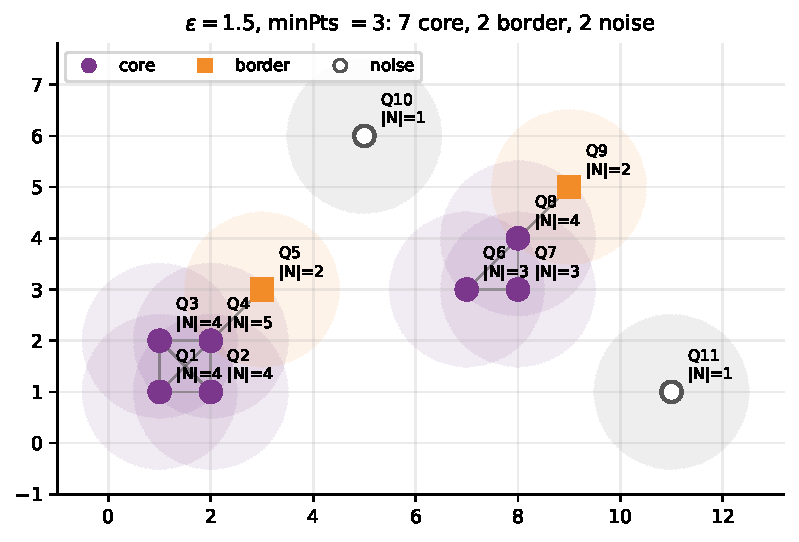
\includegraphics[width=0.82\textwidth]{dbscanhand.pdf}
  \caption{The eleven points with their $\varepsilon$-balls. Grey edges join
    pairs within $\varepsilon$; filled circles are core, squares are border,
    hollow circles are noise. $Q_{10}$ is only $3.606$ from both clusters but
    $\varepsilon = 1.5$, and that is all that matters.}
  \label{fig:dbscanhand}
\end{figure}

\subsection{The library agrees}

\begin{lstlisting}
db = DBSCAN(eps=1.5, min_samples=3).fit(P11)
print(db.labels_)
print(sorted(db.core_sample_indices_))
\end{lstlisting}
\begin{codeout}
sklearn labels_       [ 0  0  0  0  0  1  1  1  1 -1 -1]
hand labels           [ 0  0  0  0  0  1  1  1  1 -1 -1]
agree (up to renaming): True
sklearn core points   ['Q1', 'Q2', 'Q3', 'Q4', 'Q6', 'Q7', 'Q8']
hand core points      ['Q1', 'Q2', 'Q3', 'Q4', 'Q6', 'Q7', 'Q8']
identical: True
\end{codeout}

\begin{caution}[$-1$ is not a cluster index]
\texttt{DBSCAN.labels\_} uses $-1$ for noise. \texttt{np.bincount} will raise
on it, \texttt{len(set(labels))} over-counts the clusters by one, and
\texttt{adjusted\_rand\_score} will treat all the noise points as though they
formed one cluster --- which sometimes flatters the score badly. The idiom is
\texttt{n\_clusters = len(set(labels)) - (1 if -1 in labels else 0)}.
\end{caution}

\subsection{Both parameters are cliffs, not dials}

\begin{codeout}
  min_samples = 2  ->  2 clusters, 2 noise, labels [0,0,0,0,0,1,1,1,1,-1,-1]
  min_samples = 3  ->  2 clusters, 2 noise, labels [0,0,0,0,0,1,1,1,1,-1,-1]
  min_samples = 4  ->  2 clusters, 2 noise, labels [0,0,0,0,0,1,1,1,1,-1,-1]
  min_samples = 5  ->  1 clusters, 6 noise, labels [0,0,0,0,0,-1,-1,-1,-1,-1,-1]

  eps = 1.0  ->  2 clusters, 4 noise, labels [0,0,0,0,-1,1,1,1,-1,-1,-1]
  eps = 1.4  ->  2 clusters, 4 noise, labels [0,0,0,0,-1,1,1,1,-1,-1,-1]
  eps = 1.5  ->  2 clusters, 2 noise, labels [0,0,0,0,0,1,1,1,1,-1,-1]
  eps = 2.5  ->  2 clusters, 2 noise, labels [0,0,0,0,0,1,1,1,1,-1,-1]
  eps = 4.5  ->  1 clusters, 0 noise, labels [0,0,0,0,0,0,0,0,0,0,0]
\end{codeout}

Going from $\varepsilon = 1.4$ to $1.5$ crosses $\sqrt{2} = 1.4142$ and turns
the two border points into cluster members. Going from minPts $= 4$ to $5$
destroys the right-hand cluster entirely, because its core points had exactly
three and four neighbours. Small parameter changes produce discrete, not
gradual, changes in the answer.

\subsection{What DBSCAN buys: shape, $k$, and noise}

Recall Figure~\ref{fig:assumptions}. On the same four data sets where
$k$-means scored $0.274$, $-0.002$, $-0.001$ and $0.288$:

\begin{codeout}
  data                    eps  minPts   ARI    clusters  noise
  two moons              0.20     5     1.000      2        0
  concentric circles     0.18     5     1.000      2        0
  two long thin bands    0.60     5     1.000      2        0
  very unequal sizes     0.85     5     0.857      3       19
\end{codeout}

Three perfect scores on shapes that are, for $k$-means, impossible. And $k$
was discovered rather than supplied:

\begin{codeout}
blobs of 120 points, sd 0.55, centres equally spaced on a circle of radius 8;
eps = 0.45 and minPts = 5 held fixed throughout
  true k = 2  ->  DBSCAN found 2   ARI 0.9265   noise  9
  true k = 3  ->  DBSCAN found 3   ARI 0.9537   noise 11
  true k = 5  ->  DBSCAN found 5   ARI 0.9611   noise 18
  true k = 8  ->  DBSCAN found 8   ARI 0.9667   noise 26
\end{codeout}

Finally, the noise label is a deliverable in its own right. Three clean blobs
of $300$ points with $60$ points scattered uniformly over the plot:

\begin{codeout}
  planted noise points: 60   DBSCAN called 57 points noise
  of the planted noise, correctly flagged: 55 (91.7%)
  of the genuine points, wrongly flagged:   2 (0.7%)
  ARI on the 300 real points: DBSCAN 0.9901   k-means 1.0000
  k-means put all 60 planted noise points inside a cluster: it has
  no way to say 'this point does not belong to anything'.
\end{codeout}

Be honest about that last comparison: $k$-means scored slightly \emph{better}
on the real points. What it cannot do is the other half of the job. Every one
of the $60$ contaminating points was placed in a cluster and given a label as
confident as any other. DBSCAN identified $92\%$ of them at a cost of two
false positives out of $300$.

% =========================================================================
\section{DBSCAN's weakness: one global $\varepsilon$}
\label{sec:eps}

\subsection{Two densities, one radius}

$\varepsilon$ and minPts together define a single density threshold ---
roughly, minPts points per ball of radius $\varepsilon$. One threshold cannot
describe two densities, and here is a data set that makes the point
unarguable: two \emph{tight} clusters of $150$ points with standard deviation
$0.12$ whose centres are only $1.0$ apart, plus one \emph{loose} cluster of
$150$ points with standard deviation $1.60$, well away from both.

\begin{codeout}
   eps  clusters  noise |  tight A            tight B            loose C
  0.06       2     183 |  20 noise, 1 part   13 noise, 1 part  150 noise, 0 parts
  0.10       2     158 |   4 noise, 1 part    4 noise, 1 part  150 noise, 0 parts
  0.15       2     152 |   0 noise, 1 part    2 noise, 1 part  150 noise, 0 parts
  0.25       6     127 |   0 noise, 1 part    0 noise, 2 parts 127 noise, 4 parts  WELDED
  0.35       9      81 |   0 noise, 1 part    0 noise, 1 part   81 noise, 8 parts  WELDED
  0.50       4      54 |   0 noise, 1 part    0 noise, 1 part   54 noise, 3 parts  WELDED
  0.80       2      18 |   0 noise, 1 part    0 noise, 1 part   18 noise, 1 part   WELDED
  1.20       1       3 |   0 noise, 1 part    0 noise, 1 part    3 noise, 1 part   WELDED
\end{codeout}

Read it from both ends. At $\varepsilon \le 0.15$ the two tight clusters are
recovered perfectly and \emph{all $150$ points} of the loose cluster are
noise. By $\varepsilon = 0.25$ the loose cluster has barely begun to appear
(still $127$ of its $150$ points are noise, in four fragments) and the two
tight clusters have already been welded into one. There is no window.

\begin{figure}[htbp]
  \centering
  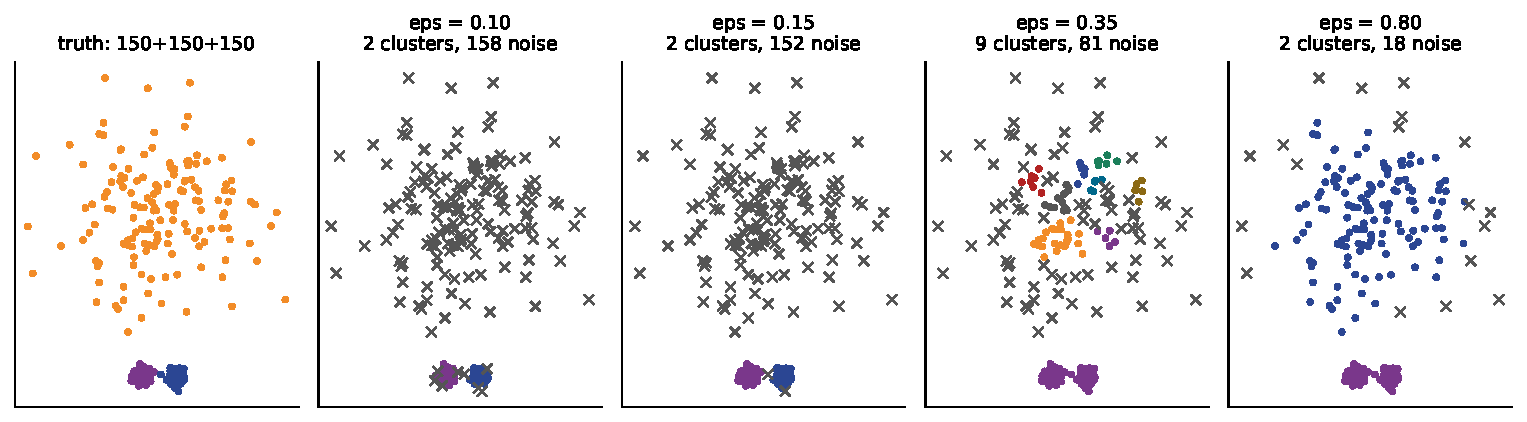
\includegraphics[width=0.94\textwidth]{density.pdf}
  \caption{The truth, then DBSCAN at $\varepsilon = 0.10, 0.15, 0.35, 0.80$.
    Grey crosses are noise. The loose cluster only appears after the two
    tight ones have merged.}
  \label{fig:density}
\end{figure}

\begin{caution}[This is not a $k$-means opportunity]
$k$-means with $k = 3$ on the same data scores ARI $0.3937$: it splits the
loose cluster and merges the tight pair. Neither method handles varying
density. The right answers are \textbf{OPTICS}, which computes a
reachability plot over a range of $\varepsilon$ instead of committing to one,
and \textbf{HDBSCAN}, which builds a hierarchy of DBSCAN results and extracts
the most stable clusters. Both are in scikit-learn
(\texttt{sklearn.cluster.OPTICS} and \texttt{sklearn.cluster.HDBSCAN}). They
are beyond this syllabus, but knowing they exist and why is worth a mark.
\end{caution}

\subsection{Choosing $\varepsilon$: the $k$-distance graph}

The standard method comes from the original paper, \S4.2. Fix minPts. For
every point compute the distance to its $(\text{minPts}-1)$-th nearest
neighbour --- equivalently, the smallest radius at which that point would be
core. Sort those $n$ numbers and plot them. Points inside a cluster have small
values; noise points have large ones. The curve therefore rises slowly and
then turns sharply upward, and the \textbf{knee} is a reasonable
$\varepsilon$.

\begin{lstlisting}
nn = NearestNeighbors(n_neighbors=5).fit(X)
dist, _ = nn.kneighbors(X)
kd = np.sort(dist[:, 4])            # distance to the 5th nearest, incl. self
plt.plot(kd)
\end{lstlisting}
\begin{codeout}
sorted 5th-nearest-neighbour distances, two moons, n = 400:
    0% quantile  0.0196     75% quantile  0.0837
   10% quantile  0.0445     90% quantile  0.1051
   25% quantile  0.0527     95% quantile  0.1179
   50% quantile  0.0642     99% quantile  0.1489
                           100% quantile  0.1665
knee (largest drop of the curve below its chord) at index 321 of 400,
eps = 0.0875
\end{codeout}

Now check what each of those candidates actually does:

\begin{codeout}
   eps   clusters  noise    ARI
  0.060     31       121    0.031
  0.080     13        41    0.185
  0.087      7        24    0.320    <-- the automatic chord knee
  0.100      4        10    0.731
  0.105      4         5    0.744    <-- 90th percentile
  0.118      3         2    0.921    <-- 95th percentile
  0.150      2         0    1.000
  0.200      2         0    1.000
  0.250      2         0    1.000
  0.270      1         0    0.000
  0.300      1         0    0.000
\end{codeout}

\begin{figure}[htbp]
  \centering
  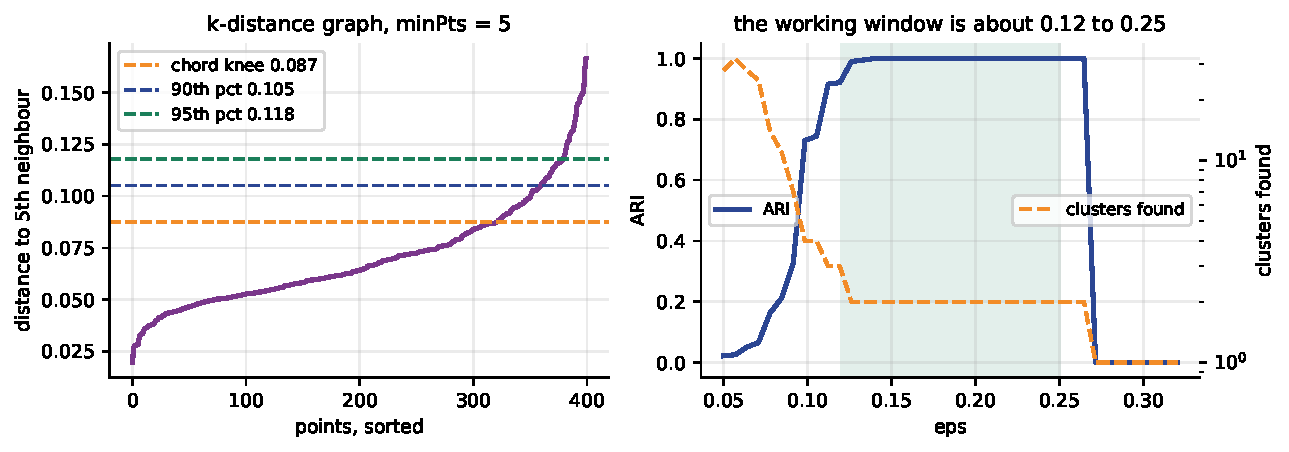
\includegraphics[width=0.90\textwidth]{kdist.pdf}
  \caption{Left: the sorted $5$-nearest-neighbour distances, with three
    candidate readings of the knee. Right: ARI (blue) and the number of
    clusters found (orange, log scale) against $\varepsilon$; the shaded band
    is the working window.}
  \label{fig:kdist}
\end{figure}

The automatic knee, at $0.0875$, gives \emph{seven} clusters and ARI $0.320$.
The $90$th and $95$th percentiles of the same curve, $0.1051$ and $0.1179$,
are much better. The original paper is candid about this: it says finding the
knee automatically is very difficult and proposes an \textbf{interactive}
procedure in which the analyst looks at the graph.

\begin{keyidea}
The $k$-distance graph converts ``choose a positive real number'' into
``choose something between about $0.09$ and $0.17$'', and then you look at
the result. It narrows the search. It does not end it.
\end{keyidea}

\subsection{How sensitive is that, exactly?}

From the table: the working window on two moons is roughly $0.12$ to $0.25$
--- a factor of two. Just below it, $\varepsilon = 0.08$ gives thirteen
clusters. Just above it, $\varepsilon = 0.27$ gives one. Between $0.25$ and
$0.27$ --- an $8\%$ change --- the answer goes from perfect to worthless.

Rules of thumb worth writing down:

\begin{itemize}[leftmargin=*]
  \item \textbf{Scale your features first.} $\varepsilon$ is a distance. One
    column measured in rupees and another in metres makes it meaningless.
  \item \textbf{minPts $\ge d + 1$}, and commonly $2d$, where $d$ is the
    number of features. Ester et al.\ used $4$ for two-dimensional data.
    Larger minPts means more points called noise and a more robust result.
  \item \textbf{Choose minPts first, then $\varepsilon$}, because the
    $k$-distance graph depends on minPts.
  \item \textbf{Look at the result.} Number of clusters, fraction of noise,
    and a two-dimensional projection. If $80\%$ of your data is noise,
    $\varepsilon$ is too small; if you have one cluster, it is too large.
\end{itemize}

\subsection{And in high dimensions it stops working altogether}

\begin{codeout}
  d      median 5-NN distance   ratio max/min NN distance
    2            0.1742              300.4036
    5            1.0580                9.6541
   10            2.3147                3.2597
   20            4.1659                2.4595
   50            7.8523                1.6474
  100           12.0239                1.3444
\end{codeout}

The right-hand column is the important one. In two dimensions the most
isolated of $500$ Gaussian points is $300$ times further from its nearest
neighbour than the most crowded one is; at $d = 100$ that ratio is $1.34$.
Every point is about equally far from every other point, so no single radius
separates ``dense'' from ``sparse''. This is the concentration-of-distances
phenomenon, and it is fatal for any method whose parameter is an absolute
distance.

It shows up immediately on real data. Setting $\varepsilon$ automatically to
the $90$th percentile of the $2d$-nearest-neighbour distance --- the
$k$-distance heuristic applied without human judgement --- gives:

\begin{codeout}
  data            n     d   k   k-means ARI  k-medoids ARI  DBSCAN ARI  DBSCAN k  noise
  iris            150     4   3       0.6201        0.6416      0.5438       2       4
  wine            178    13   3       0.8975        0.7411     -0.0074       1       5
  breast cancer   569    30   2       0.6536        0.6079      0.0200       1      13
  digits         1797    64  10       0.4679        0.3854      0.0002       1      45
\end{codeout}

DBSCAN finds \emph{one} cluster on wine, breast cancer and digits. That is not
a tuning failure to be fixed by trying harder; it is the geometry. On
moderately high-dimensional numeric data, reduce the dimension first (PCA,
UMAP) or use a partitioning method.

% =========================================================================
\section{Choosing between them}
\label{sec:choose}

\begin{center}\small
\begin{tabular}{lllll}
  \toprule
   & $k$-means & $k$-medoids (PAM) & CLARA & DBSCAN \\
  \midrule
  supply $k$?      & yes & yes & yes & \textbf{no} \\
  representative   & the mean & a data object & a data object & none \\
  dissimilarity    & squared Euclidean & \textbf{any} & \textbf{any} & any \\
  cluster shape    & convex & convex & convex & \textbf{arbitrary} \\
  outliers         & drag the mean & robust-ish & robust-ish
                   & \textbf{labelled} \\
  deterministic    & no & \textbf{yes} & no & yes* \\
  time             & $O(nkdi)$ & $O(k(n{-}k)^2)$/iter
                   & $O(ks^2 + k(n{-}k))$ & $O(n\log n)$ indexed \\
  memory           & $O(nd)$ & $O(n^2)$ & $O(s^2 + n)$ & $O(n)$ \\
  practical $n$    & millions & thousands & millions & millions \\
  \bottomrule
\end{tabular}
\end{center}

\noindent{\small *except for border points within $\varepsilon$ of two
clusters, which are assigned by visiting order.}

\begin{codeout}
  measured at n = 200,000, k = 5:
    k-means (n_init = 10)   0.270 s
    CLARA   (5 x 50)        0.065 s
    DBSCAN  (eps = 0.30)    5.745 s
    PAM     the distance matrix alone is 298.0 GiB
    HAC     the condensed matrix alone is 149.0 GiB
\end{codeout}

A short decision procedure that will serve you in the lab:

\begin{enumerate}[leftmargin=*]
  \item \textbf{Do you know $k$, or can you defend a choice of it?} If not,
    and the data is low-dimensional, start with DBSCAN. If not, and the data
    is high-dimensional, use hierarchical clustering and look at the tree.
  \item \textbf{Is your dissimilarity Euclidean, and can you average your
    objects?} If not, $k$-means is unavailable; use $k$-medoids (or CLARA at
    scale), or hierarchical clustering with average or complete linkage.
  \item \textbf{Do you expect non-convex clusters?} Then not $k$-means, not
    $k$-medoids, not CLARA. DBSCAN, or single-linkage hierarchical
    clustering.
  \item \textbf{Do you have outliers, and do they matter?} $k$-means is the
    worst choice; $k$-medoids is much better; DBSCAN labels them for you.
  \item \textbf{How large is $n$?} Under a few thousand, anything. Tens of
    thousands, not PAM and not hierarchical. Hundreds of thousands,
    $k$-means, CLARA or indexed DBSCAN.
  \item \textbf{Whatever you choose, scale the features first}, and record
    the random seed.
\end{enumerate}

% =========================================================================
\section{Summary}
\label{sec:summary}

\begin{enumerate}[leftmargin=*]
  \item A \textbf{partitioning} method takes $k$ and returns one partition.
    $k$-means minimises
    $\mathrm{WCSS} = \sum_j\sum_{x \in C_j}\lVert x - c_j\rVert^2$.
  \item \textbf{Lloyd's algorithm}: assign each point to the nearest
    centroid, move each centroid to the mean of its cluster, repeat until
    nothing changes.
  \item The hand run on seven points: $123 \to 32.2 \to 16.74 \to 11.4167$,
    converged in three iterations, one point ($P_3$) changing cluster ---
    and confirmed against \texttt{KMeans} to $10^{-12}$.
  \item \textbf{Both steps are non-increasing} in the objective (the mean
    minimises the sum of squared distances, equation~\eqref{eq:meanlemma})
    and there are finitely many partitions, so the algorithm terminates ---
    at a \textbf{local} optimum.
  \item Twenty random starts on one data set gave \textbf{twelve} different
    answers, the worst $11.6\times$ the best.
    \textbf{$k$-means\texttt{++}} reaches the best on $99.5\%$ of single
    starts against $32\%$ for uniform random seeding; \texttt{n\_init=10}
    with random seeding reaches $97.5\%$.
  \item Never report a $k$-means result from a single random start. Record
    the seed.
  \item \textbf{Elbow and silhouette are heuristics.} On iris the chord
    elbow says $3$, the drop-ratio elbow says $2$, the silhouette says $2$
    and the species say $3$. On $500$ uniform random points the silhouette
    still peaks, at $k = 4$.
  \item $k$-means assumes \textbf{spherical, similar-sized, similar-density}
    clusters. ARI $0.274$ on two moons, $-0.001$ on two long bands, and a
    $400/40/40$ truth returned as $208/176/96$.
  \item \textbf{The mean is not robust}: one point at $(12,9)$ moves a
    centroid by $2.15$ and changes the partition; two outliers in $302$
    points take $k$-means from ARI $1.000$ to $0.000$.
  \item \textbf{$k$-medoids} minimises $E = \sum_j\sum_{x \in C_j} d(x,o_j)$
    with $o_j$ an actual object and $d$ any dissimilarity. Unaffected by
    those two outliers; clusters words by edit distance, where $k$-means is
    undefined.
  \item \textbf{PAM} is BUILD then SWAP; one SWAP iteration is
    $O(k(n-k)^2)$ and it needs $O(n^2)$ memory. Measured: $98\times$ slower
    than $k$-means at $n = 4000$, growth exponent $2.34$.
  \item \textbf{CLARA} samples $40+2k$ objects, runs PAM on the sample,
    assigns all $n$, repeats five times and keeps the best. It does $1576$
    times less swap work than PAM at $n = 4000$ for $4.4\%$ more cost ---
    but randomised, with a $5.3\%$ cost spread over ten seeds.
  \item \textbf{DBSCAN} needs $\varepsilon$ and minPts, not $k$. A point is
    \textbf{core} if $|N_\varepsilon(p)| \ge$ minPts, \textbf{border} if it
    is in a core point's neighbourhood, \textbf{noise} otherwise; a cluster
    is a maximal density-connected set.
  \item The hand run on eleven points: $7$ core, $2$ border, $2$ noise,
    $2$ clusters --- identical to \texttt{DBSCAN(eps=1.5, min\_samples=3)}.
  \item DBSCAN scores ARI $1.000$ on moons, circles and two long bands where
    $k$-means scores $0.274$, $-0.002$ and $-0.001$; it discovers $k$
    ($2,3,5,8$ correctly with fixed parameters); and it flags $95\%$ of
    planted noise.
  \item \textbf{One global $\varepsilon$ cannot serve two densities.} On the
    tight/tight/loose data set, every $\varepsilon$ either leaves the loose
    cluster entirely as noise or welds the two tight clusters together.
    OPTICS and HDBSCAN exist for this.
  \item The \textbf{$k$-distance graph} narrows $\varepsilon$ to a region and
    no further; the working window on two moons is a factor of two wide, with
    thirteen clusters just below it and one just above.
  \item In $30$ or $64$ dimensions DBSCAN with a heuristically chosen
    $\varepsilon$ finds \textbf{one} cluster, because the ratio of the
    largest to the smallest nearest-neighbour distance falls from $300$ at
    $d = 2$ to $1.34$ at $d = 100$.
\end{enumerate}

% =========================================================================
\section{Practice questions}
\label{sec:practice}

\begin{enumerate}[leftmargin=*, label=\textbf{Q\arabic*.}]
  \item \textbf{(By hand.)} Six points:
    $A(1,1)$, $B(2,1)$, $C(1,2)$, $D(6,5)$, $E(7,5)$, $F(6,6)$. Run
    $k$-means with $k = 2$ from the initial centroids $c_1 = A = (1,1)$ and
    $c_2 = B = (2,1)$. Write out the distance table at every assignment step,
    the new means at every update step, and the WCSS after \emph{every half
    step}, until nothing changes. State the final clusters and the final
    WCSS.

  \item \textbf{(By hand.)} Same six points, same $k = 2$, but start from
    $c_1 = A = (1,1)$ and $c_2 = C = (1,2)$. Does the algorithm reach the same
    answer? Now start from $c_1 = (3.5, 3.5)$ and $c_2 = (3.5, 3.6)$ and do
    the first iteration only. What does this tell you about the role of the
    initial centroids?

  \item \textbf{(By hand.)} Nine points:
    $R_1(0,0)$, $R_2(1,0)$, $R_3(0,1)$, $R_4(1,1)$, $R_5(2,2)$, $R_6(5,0)$,
    $R_7(6,0)$, $R_8(6,1)$, $R_9(9,4)$. With $\varepsilon = 1.5$ and
    minPts $= 3$ (counting the point itself), list $N_\varepsilon(p)$ for
    every point, classify each as core, border or noise, and give the
    clusters and the noise set.

  \item \textbf{(By hand.)} Take the same nine points and change
    $\varepsilon$ to $1.0$, keeping minPts $= 3$. Reclassify every point.
    Then change minPts to $4$ with $\varepsilon = 1.5$ and reclassify again.
    Summarise in one sentence what each parameter controls.

  \item \textbf{(By hand.)} For the six points of Q1, compute the
    $k$-medoids cost $E$ for the medoid pairs $\{A, D\}$, $\{A, E\}$ and
    $\{B, E\}$. Which is best of the three? Starting from $\{A, B\}$,
    perform one SWAP step: which single swap reduces $E$ the most, and by
    how much?

  \item You have $250{,}000$ transaction records and want $k = 8$ medoids.
    Compute (a) the number of candidate swap evaluations in one PAM SWAP
    iteration, and (b) the size in GiB of the float64 dissimilarity matrix
    PAM requires. Then state the sample size CLARA would use under the
    standard rule, and the size of the matrix it needs.

  \item Prove that for a finite set $S$ with mean $\bar{x}$ and any point
    $z$, $\sum_{x \in S}\lVert x - z\rVert^2
    = \sum_{x \in S}\lVert x - \bar{x}\rVert^2 + |S|\lVert\bar{x}-z\rVert^2$.
    Then use it to say, in two sentences, why the update step of $k$-means
    cannot increase the objective and why $k$-means uses the mean rather than
    the median.

  \item A colleague runs $k$-means with $k$ from $2$ to $10$ on a data set,
    reports that the silhouette is maximised at $k = 3$ with a value of
    $0.41$, and concludes that the data has three clusters. Give three
    specific checks you would ask them to run before accepting that
    conclusion, and say what each one would rule out.

  \item For each of the following, name the method you would use and give one
    sentence of justification.
    (a) $2{,}000$ protein sequences with a precomputed pairwise alignment-score
    dissimilarity, and you want five representative sequences.
    (b) $800{,}000$ GPS pings, and you want to find the places where vehicles
    stop, without knowing how many places there are.
    (c) $50{,}000$ standardised customer rows with $12$ numeric features,
    known to contain data-entry errors with impossible values.
    (d) $400$ gene-expression profiles where you want to inspect structure at
    several granularities before committing to a number of groups.

  \item DBSCAN on a two-dimensional data set with $\varepsilon = 0.5$ and
    minPts $= 5$ returns $1$ cluster and $0$ noise points. With
    $\varepsilon = 0.1$ it returns $47$ clusters and $612$ noise points out of
    $1000$. Describe exactly what you would do next, in order, and what
    result would make you conclude that DBSCAN is the wrong method for this
    data.
\end{enumerate}

% =========================================================================
\section{Solutions}
\label{sec:solutions}

\paragraph{Q1 --- the $k$-means run, worked in full.}
Points $A(1,1)$, $B(2,1)$, $C(1,2)$, $D(6,5)$, $E(7,5)$, $F(6,6)$;
$c_1 = (1,1)$, $c_2 = (2,1)$.

\textbf{Iteration 1, assignment.}
\[
\begin{array}{lccl}
  & d(\cdot,c_1) & d(\cdot,c_2) & \\[2pt]
  A(1,1) & 0.0000 & 1.0000 & C_1\\
  B(2,1) & 1.0000 & 0.0000 & C_2\\
  C(1,2) & 1.0000 & \sqrt{2}=1.4142 & C_1\\
  D(6,5) & \sqrt{25+16}=6.4031 & \sqrt{16+16}=5.6569 & C_2\\
  E(7,5) & \sqrt{36+16}=7.2111 & \sqrt{25+16}=6.4031 & C_2\\
  F(6,6) & \sqrt{25+25}=7.0711 & \sqrt{16+25}=6.4031 & C_2
\end{array}
\]
$C_1 = \{A,C\}$, $C_2 = \{B,D,E,F\}$.
WCSS $= (0 + 1) + (0 + 32 + 41 + 41) = 1 + 114 = \mathbf{115.0000}$.

\textbf{Iteration 1, update.}
$c_1 = \frac12(1{+}1,\ 1{+}2) = (1.0,\ 1.5)$;
$c_2 = \frac14(2{+}6{+}7{+}6,\ 1{+}5{+}5{+}6) = \bigl(\frac{21}{4},
\frac{17}{4}\bigr) = (5.25,\ 4.25)$.
WCSS $= (0.25 + 0.25) + (13.5625 + 1.125 + 3.625 + 3.625)
= 0.5 + 21.9375 = \mathbf{22.4375}$.

\textbf{Iteration 2, assignment.}
\[
\begin{array}{lccl}
  & d(\cdot,c_1) & d(\cdot,c_2) & \\[2pt]
  A(1,1) & 0.5000 & \sqrt{18.0625+10.5625}=5.3502 & C_1\\
  B(2,1) & \sqrt{1+0.25}=1.1180 & \sqrt{10.5625+10.5625}=4.5962 & C_1\ \text{--- moved}\\
  C(1,2) & 0.5000 & \sqrt{18.0625+5.0625}=4.8088 & C_1\\
  D(6,5) & \sqrt{25+12.25}=6.1033 & \sqrt{0.5625+0.5625}=1.0607 & C_2\\
  E(7,5) & \sqrt{36+12.25}=6.9462 & \sqrt{3.0625+0.5625}=1.9039 & C_2\\
  F(6,6) & \sqrt{25+20.25}=6.7268 & \sqrt{0.5625+3.0625}=1.9039 & C_2
\end{array}
\]
$C_1 = \{A,B,C\}$, $C_2 = \{D,E,F\}$.
WCSS $= (0.25 + 1.25 + 0.25) + (1.125 + 3.625 + 3.625)
= 1.75 + 8.375 = \mathbf{10.1250}$.

\textbf{Iteration 2, update.}
$c_1 = \frac13(1{+}2{+}1,\ 1{+}1{+}2) = \bigl(\frac43, \frac43\bigr)
= (1.3333,\ 1.3333)$;
$c_2 = \frac13(6{+}7{+}6,\ 5{+}5{+}6) = \bigl(\frac{19}{3}, \frac{16}{3}\bigr)
= (6.3333,\ 5.3333)$.
WCSS: for $C_1$, $A$ contributes $2\times(1/3)^2 = 0.2222$, $B$ contributes
$(2/3)^2 + (1/3)^2 = 0.5556$, $C$ contributes $(1/3)^2 + (2/3)^2 = 0.5556$,
total $\frac43 = 1.3333$. By symmetry $C_2$ also gives $\frac43 = 1.3333$.
Total $= \mathbf{2.6667}$.

\textbf{Iteration 3, assignment.} $A$, $B$, $C$ are all within $0.75$ of
$c_1$ and more than $6$ from $c_2$; $D$, $E$, $F$ are all within $0.75$ of
$c_2$ and more than $6$ from $c_1$. Nothing changes, so the algorithm stops.

\textbf{Answer.} $C_1 = \{A,B,C\}$, $C_2 = \{D,E,F\}$, final WCSS
$= \mathbf{2.6667}$. The sequence of half-step values is
$115 \to 22.4375 \to 10.125 \to 2.6667 \to 2.6667$, non-increasing throughout,
as it must be.

\paragraph{Q2 --- initialisation.}
From $c_1 = A = (1,1)$, $c_2 = C = (1,2)$: at iteration~1, $A$ and $B$ go to
$C_1$ (since $d(B,c_1) = 1 < d(B,c_2) = \sqrt{2}$) and $C$, $D$, $E$, $F$ go
to $C_2$. The update gives $c_1 = (1.5, 1)$ and
$c_2 = \frac14(1{+}6{+}7{+}6,\ 2{+}5{+}5{+}6) = (5, 4.5)$. At iteration~2,
$C(1,2)$ is $\sqrt{0.25+1} = 1.1180$ from $c_1$ and $\sqrt{16+6.25} = 4.7170$
from $c_2$, so it returns to $C_1$; nothing else moves. Update gives
$c_1 = (1.3333, 1.3333)$, $c_2 = (6.3333, 5.3333)$, and iteration~3 changes
nothing. \textbf{Same answer as Q1}, WCSS $2.6667$.

From $c_1 = (3.5, 3.5)$, $c_2 = (3.5, 3.6)$: every point is assigned by the
$y$-coordinate alone, because the two centroids differ only in $y$. Points
with $y < 3.55$ --- $A$, $B$, $C$ --- are closer to $c_1$; points with
$y > 3.55$ --- $D$, $E$, $F$ --- are closer to $c_2$. So the very first
assignment is already the correct one and the run converges immediately.

\textbf{What it tells you.} On six points in two obvious clumps almost any
start works, and that is exactly why a small clean example cannot demonstrate
the initialisation problem. The failure mode needs several clusters and a
start that puts two centroids inside one of them, which is what the $600$-point
six-blob experiment in Section~\ref{sec:conv} does: twelve distinct answers
from twenty seeds.

\paragraph{Q3 --- DBSCAN on nine points, $\varepsilon = 1.5$, minPts $= 3$.}
Distances inside $\varepsilon$: grid steps of $1$ and diagonals of
$\sqrt{2} = 1.4142$. Everything else ($2$, $\sqrt{5} = 2.236$, and up) is
outside.

\[
\begin{array}{llrl}
  \text{point} & N_\varepsilon(p) & |N| & \text{verdict}\\[2pt]
  R_1(0,0) & \{R_1,R_2,R_3,R_4\} & 4 & \text{CORE}\\
  R_2(1,0) & \{R_1,R_2,R_3,R_4\} & 4 & \text{CORE}\\
  R_3(0,1) & \{R_1,R_2,R_3,R_4\} & 4 & \text{CORE}\\
  R_4(1,1) & \{R_1,R_2,R_3,R_4,R_5\} & 5 & \text{CORE}\\
  R_5(2,2) & \{R_4,R_5\} & 2 & \text{BORDER}\\
  R_6(5,0) & \{R_6,R_7\} & 2 & \text{not core}\\
  R_7(6,0) & \{R_6,R_7,R_8\} & 3 & \text{CORE}\\
  R_8(6,1) & \{R_7,R_8\} & 2 & \text{not core}\\
  R_9(9,4) & \{R_9\} & 1 & \text{NOISE}
\end{array}
\]
Check the ones that are easy to get wrong: $d(R_4,R_5) = \sqrt{1+1} = 1.4142
\le 1.5$, so $R_5$ is in $N_\varepsilon(R_4)$ and $R_4$ is core, making $R_5$
a border point. $d(R_6,R_8) = \sqrt{1+1} = 1.4142 \le 1.5$, so
$N_\varepsilon(R_7) = \{R_6,R_7,R_8\}$ has size $3$ and $R_7$ is core; but
$N_\varepsilon(R_6) = \{R_6,R_7\}$ and $N_\varepsilon(R_8) = \{R_7,R_8\}$
each have size $2$, so $R_6$ and $R_8$ are \textbf{border} points of $R_7$'s
cluster. $d(R_5,R_6) = \sqrt{9+4} = 3.606 > 1.5$, so the two groups do not
connect.

\textbf{Answer.} Core: $R_1,R_2,R_3,R_4,R_7$. Border: $R_5,R_6,R_8$. Noise:
$R_9$. Clusters: $\{R_1,R_2,R_3,R_4,R_5\}$ and $\{R_6,R_7,R_8\}$. Two
clusters, one noise point.

\paragraph{Q4 --- the same points with different parameters.}
\textbf{$\varepsilon = 1.0$, minPts $= 3$.} Now only the grid steps of $1$
count; $\sqrt{2}$ is out. $N_\varepsilon(R_1) = \{R_1,R_2,R_3\}$ (size 3,
core), $N_\varepsilon(R_2) = \{R_1,R_2,R_4\}$ (core),
$N_\varepsilon(R_3) = \{R_1,R_3,R_4\}$ (core),
$N_\varepsilon(R_4) = \{R_2,R_3,R_4\}$ (core).
$N_\varepsilon(R_5) = \{R_5\}$: \textbf{noise}, since it is now in nobody's
ball. $N_\varepsilon(R_6) = \{R_6,R_7\}$ (2), $N_\varepsilon(R_7) =
\{R_6,R_7,R_8\}$ (3, core), $N_\varepsilon(R_8) = \{R_7,R_8\}$ (2). So
$R_6, R_8$ remain border points of $R_7$. $R_9$ is still noise.
\textbf{Result:} clusters $\{R_1,R_2,R_3,R_4\}$ and $\{R_6,R_7,R_8\}$; noise
$\{R_5, R_9\}$.

\textbf{$\varepsilon = 1.5$, minPts $= 4$.} Recount the neighbourhood sizes
from Q3 against the new threshold of $4$: $R_1$ (4, core), $R_2$ (4, core),
$R_3$ (4, core), $R_4$ (5, core), $R_5$ (2, border of $R_4$), $R_6$ (2),
$R_7$ (\textbf{3}, no longer core), $R_8$ (2), $R_9$ (1). The right-hand
group now has \emph{no} core point at all, so all of $R_6, R_7, R_8$ become
noise. \textbf{Result:} one cluster $\{R_1,R_2,R_3,R_4,R_5\}$; noise
$\{R_6,R_7,R_8,R_9\}$.

\textbf{One sentence each.} $\varepsilon$ sets how far a point may reach to
find neighbours, so lowering it fragments clusters and turns marginal points
into noise; minPts sets how many neighbours a point needs to be allowed to
grow a cluster, so raising it destroys sparse clusters wholesale by removing
their core points.

\paragraph{Q5 --- $k$-medoids on the six points.}
The distances needed:
$d(A,B) = 1$, $d(A,C) = 1$, $d(B,C) = \sqrt{2} = 1.4142$,
$d(D,E) = 1$, $d(D,F) = 1$, $d(E,F) = \sqrt{1+1} = 1.4142$,
$d(A,D) = \sqrt{25+16} = 6.4031$, $d(A,E) = \sqrt{36+16} = 7.2111$,
$d(B,D) = \sqrt{16+16} = 5.6569$, $d(B,E) = \sqrt{25+16} = 6.4031$,
$d(C,D) = \sqrt{25+9} = 5.8310$, $d(C,E) = \sqrt{36+9} = 6.7082$.

$\{A,D\}$: $A \to 0$; $B \to \min(1,\ 5.6569) = 1$;
$C \to \min(1,\ 5.8310) = 1$; $D \to 0$; $E \to \min(7.2111,\ 1) = 1$;
$F \to \min(\sqrt{25+25},\ 1) = 1$. \quad
$E_{\{A,D\}} = 0+1+1+0+1+1 = \mathbf{4.0000}$.

$\{A,E\}$: $A \to 0$; $B \to 1$; $C \to 1$; $D \to \min(6.4031, 1) = 1$;
$E \to 0$; $F \to \min(7.0711,\ 1.4142) = 1.4142$. \quad
$E_{\{A,E\}} = \mathbf{4.4142}$.

$\{B,E\}$: $A \to \min(1,\ 7.2111) = 1$; $B \to 0$; $C \to \min(1.4142,
6.7082) = 1.4142$; $D \to 1$; $E \to 0$; $F \to 1.4142$. \quad
$E_{\{B,E\}} = \mathbf{4.8284}$.

\textbf{Best of the three: $\{A,D\}$ with $E = 4.0000$.}

\textbf{The SWAP step from $\{A,B\}$.} First, $E_{\{A,B\}}$: $A \to 0$,
$B \to 0$, $C \to \min(1, 1.4142) = 1$, $D \to \min(6.4031, 5.6569) = 5.6569$,
$E \to \min(7.2111, 6.4031) = 6.4031$,
$F \to \min(7.0711, \sqrt{16+25}=6.4031) = 6.4031$, giving
$E_{\{A,B\}} = 19.4631$. The candidate swaps that put a medoid on the right
are the useful ones; swapping $B \to D$ gives $E_{\{A,D\}} = 4.0000$, a change
of $-15.4631$; swapping $B \to E$ gives $4.4142$ ($-15.0489$); swapping
$B \to F$ gives, by the symmetry of $D$ and $F$ about the group,
$E_{\{A,F\}} = 0+1+1+1+1.4142+0 = 4.4142$ ($-15.0489$). Swapping
$A \to D$ gives $E_{\{B,D\}} = 1+0+1.4142+0+1+1 = 4.4142$. \textbf{The best
single swap is $B \to D$, reducing $E$ by $15.4631$ to $4.0000$.}

\paragraph{Q6 --- PAM and CLARA arithmetic at $n = 250{,}000$, $k = 8$.}
(a) $k(n-k)^2 = 8 \times (250000-8)^2 = 8 \times 249992^2
= 8 \times 6.24960\times10^{10} = \mathbf{4.9997 \times 10^{11}}$
evaluations in \emph{one} SWAP iteration.
(b) $n^2 \times 8$ bytes $= 250000^2 \times 8 = 5 \times 10^{11}$ bytes
$= 5\times10^{11} / 2^{30} = \mathbf{465.7}$\,GiB.
Both numbers rule PAM out completely.

CLARA's standard sample size is $40 + 2k = 40 + 16 = \mathbf{56}$ objects. Its
dissimilarity matrix is $56 \times 56 \times 8$ bytes $= 25{,}088$ bytes,
about $\mathbf{24.5}$\,KiB --- a factor of roughly $2 \times 10^{7}$ smaller.
The work per sample is $O(k s^2) = 8 \times 56^2 = 25{,}088$ for the PAM part,
plus $O(k(n-k)) \approx 2 \times 10^{6}$ for assigning all $n$ objects, and
that assignment sweep is what dominates.

\paragraph{Q7 --- the mean lemma.}
Write $x - z = (x - \bar{x}) + (\bar{x} - z)$ and expand the squared norm:
\[
  \lVert x-z\rVert^2 = \lVert x-\bar{x}\rVert^2
    + 2\langle x-\bar{x},\ \bar{x}-z\rangle + \lVert\bar{x}-z\rVert^2 .
\]
Sum over $x \in S$. The middle term is
$2\langle \sum_{x\in S}(x-\bar{x}),\ \bar{x}-z\rangle$, and
$\sum_{x \in S}(x - \bar{x}) = \sum_{x\in S}x - |S|\bar{x} = 0$ by the
definition of $\bar{x}$, so it vanishes. The last term does not depend on $x$
and is added $|S|$ times. \ensuremath{\square}

\textbf{Why the update step cannot increase WCSS.} For each cluster the
identity says the contribution with representative $z$ exceeds the
contribution with representative $\bar{x}$ by $|S|\lVert\bar{x}-z\rVert^2 \ge
0$. Replacing the old centroid by the mean therefore lowers (or leaves
unchanged) each cluster's contribution, hence the total.

\textbf{Why the mean and not the median.} The lemma is specifically about the
sum of \emph{squared} distances; the mean is its unique minimiser. If the
objective were the sum of unsquared distances the minimiser would be the
geometric median, which is exactly the change $k$-medoids makes --- and the
reason it is robust, since the median is not dragged by a single extreme
value while the mean is.

\paragraph{Q8 --- three checks on ``silhouette says three''.}
\textbf{Check 1: run it on a null data set of the same shape.} Draw the same
number of points uniformly (or resample each column independently, destroying
the joint structure) and compute the best silhouette. If the null data also
gives about $0.41$, the score is not evidence of structure. The notes show
$500$ uniform points reaching $0.4060$ at $k=4$. This rules out
\emph{spurious structure}.

\textbf{Check 2: look at the cluster sizes and a two-dimensional
projection.} A $998/1/1$ split scores well on some criteria and is
outlier-peeling, not clustering; a projection will also show at once whether
the clusters are elongated or crescent-shaped, in which case the silhouette
is measuring the wrong thing because it rewards compactness. This rules out
\emph{degenerate or wrong-shaped solutions}.

\textbf{Check 3: stability under resampling and reseeding.} Refit on ten
bootstrap samples or with ten \texttt{random\_state} values and compare the
partitions with the adjusted Rand index. If $k = 3$ is real, the partitions
should agree with each other. This rules out \emph{a local optimum being
mistaken for a finding}.

\paragraph{Q9 --- method selection.}
(a) \textbf{$k$-medoids (PAM)}. The dissimilarity is precomputed and
non-Euclidean, so there is no mean and $k$-means is undefined; $n = 2000$ is
small enough for PAM's $O(n^2)$ matrix ($32$\,MiB) and its $O(k(n-k)^2)$
iterations; and the requirement for ``five representative sequences'' is
literally a request for medoids.

(b) \textbf{DBSCAN}. The number of stopping places is unknown, so any method
requiring $k$ is out; stopping places are dense blobs of pings surrounded by
sparse travelling pings, which is exactly the density-based cluster
definition; and the travelling pings should be labelled noise rather than
forced into a cluster. With a spatial index this is $O(n \log n)$ at
$n = 800{,}000$.

(c) \textbf{$k$-medoids via CLARA, or $k$-means after explicit outlier
removal}. The impossible values are outliers that would drag $k$-means
centroids badly --- two outliers in $302$ points were enough to destroy it in
Section~\ref{sec:medoid} --- and $n = 50{,}000$ rules out PAM directly, so
CLARA. The better engineering answer is to clean the data first and then use
$k$-means; say so.

(d) \textbf{Hierarchical agglomerative clustering}. ``Inspect structure at
several granularities before committing'' is a description of a dendrogram.
$n = 400$ makes the $O(n^2)$ memory trivial, and the result is deterministic,
which matters when you are going to look at it and argue about it.

\paragraph{Q10 --- what to do next.}
\textbf{1.} Recognise the symptom: $\varepsilon = 0.5$ is above the welding
threshold and $\varepsilon = 0.1$ is below the connection threshold, so the
useful value is somewhere between, or does not exist.

\textbf{2.} Check the scaling first. If one feature has a range of $100$ and
the other of $0.01$, $\varepsilon$ is effectively a threshold on the first
feature alone. Standardise and repeat.

\textbf{3.} Plot the $k$-distance graph with minPts $= 5$: sort the distances
to each point's fifth nearest neighbour and look for the knee. Take the
$90$th and $95$th percentiles as bracketing candidates.

\textbf{4.} Sweep $\varepsilon$ across that bracket --- say fifteen values on
a log scale between $0.1$ and $0.5$ --- and for each record the number of
clusters, the noise fraction and the cluster sizes. Plot all three against
$\varepsilon$.

\textbf{5.} Look for a \emph{plateau}: a range of $\varepsilon$ over which
the number of clusters is stable. A real cluster structure produces one; the
two-moons example in Section~\ref{sec:eps} has a plateau of two clusters from
$0.12$ to $0.25$.

\textbf{6. What would make me abandon DBSCAN.} If the sweep shows no plateau
at all --- the count sliding monotonically from many clusters to one with no
stable region --- then there is no single density that describes the data.
Two causes, and both have a different answer. If the clusters have genuinely
different densities, use \textbf{OPTICS} or \textbf{HDBSCAN}. If the data is
high-dimensional (say $d > 10$) and the ratio of the largest to the smallest
nearest-neighbour distance is close to $1$, then no distance threshold will
work at all; reduce the dimension first or use a partitioning method.

% =========================================================================
\section{References and further reading}
\label{sec:refs}

All links were checked on 24 August 2026. Free resources are marked
\textbf{[free]}.

\subsection*{Textbooks}

\begin{itemize}[leftmargin=*]
  \item Han, Kamber and Pei, \emph{Data Mining: Concepts and Techniques}, 3rd
    edition, Morgan Kaufmann, 2012. \textbf{The prescribed text for this
    lecture.} \S10.2 partitioning methods --- \S10.2.1 is $k$-means with the
    worked figure and the complexity $O(nkt)$; \S10.2.2 is $k$-medoids, PAM
    and \textbf{CLARA}, with the $O(k(n-k)^2)$ per-iteration cost and the
    $40+2k$ sample-size rule quoted in Section~\ref{sec:clara} here. \S10.4
    is density-based methods --- \S10.4.1 is DBSCAN, with core, border and
    noise, density-reachability and density-connectivity in exactly the
    notation the examination uses; \S10.4.2 is OPTICS, the answer to
    Section~\ref{sec:eps}. \S10.6.3 is the silhouette.
  \item James, Witten, Hastie, Tibshirani and Taylor, \emph{An Introduction to
    Statistical Learning with Python}. \textbf{[free]} \S12.4.1 is $k$-means
    at a gentler pace: the objective, the algorithm, the guarantee that the
    objective decreases at every step, and --- importantly --- a figure
    showing six different local optima from six different random starts, which
    is Section~\ref{sec:conv} here. \S12.4.3 discusses the practical issues.
    \url{https://www.statlearning.com/}
  \item Kaufman and Rousseeuw, \emph{Finding Groups in Data: An Introduction
    to Cluster Analysis}, Wiley, 1990. The book that introduced PAM, CLARA
    \emph{and} the silhouette. Chapter 2 is PAM, Chapter 3 is CLARA. If you
    want the original statement of anything in Sections~\ref{sec:medoid}
    and~\ref{sec:clara}, it is here. \url{https://doi.org/10.1002/9780470316801}
  \item Manning, Raghavan and Sch\"utze, \emph{Introduction to Information
    Retrieval}, Cambridge University Press, 2008. \textbf{[free, full text
    online]} Chapter 16 is flat clustering: \S16.4 is $k$-means with a careful
    proof that the objective decreases and a discussion of seeding, \S16.4.1
    is cluster cardinality, \S16.3 is evaluation.
    \url{https://nlp.stanford.edu/IR-book/html/htmledition/flat-clustering-1.html}
  \item Hastie, Tibshirani and Friedman, \emph{The Elements of Statistical
    Learning}, 2e, Springer. \textbf{[free]} \S14.3.6 is $k$-means, \S14.3.8
    is vector quantisation, \S14.3.9 is $k$-medoids, and \S14.3.11 is the
    gap statistic --- a more principled alternative to the elbow than either
    heuristic in Section~\ref{sec:k}.
    \url{https://hastie.su.domains/ElemStatLearn/}
  \item Tan, Steinbach, Karpatne and Kumar, \emph{Introduction to Data
    Mining}. The cluster-analysis chapter is the standard source for the
    presentation of $k$-means used here, including the ``bisecting
    $k$-means'' variant and a careful treatment of DBSCAN's parameters. The
    authors' lecture slides are free.
    \url{https://www-users.cse.umn.edu/~kumar001/dmbook/index.php}
  \item M\"uller and Guido, \emph{Introduction to Machine Learning with
    Python}, O'Reilly, 2016. \S3.5.1 $k$-means (with the failure cases),
    \S3.5.3 DBSCAN. Short and practical. Notebooks \textbf{[free]}:
    \url{https://github.com/amueller/introduction_to_ml_with_python}
\end{itemize}

\subsection*{Online courses}

\begin{sloppypar}
\begin{itemize}[leftmargin=*]
  \item \textbf{NPTEL, Introduction to Machine Learning} --- Prof.\ Balaraman
    Ravindran, IIT Madras; the reference course for the semester. The
    clustering week covers $k$-means, the convergence argument and the choice
    of $k$ in the notation used here. \textbf{[free]}
    \url{https://nptel.ac.in/courses/106106139}
  \item \textbf{NPTEL, Data Mining} --- Prof.\ Pabitra Mitra, IIT Kharagpur.
    Follows the Han--Kamber--Pei chapter structure, so its clustering weeks
    map onto \S10.2 and \S10.4 directly --- including $k$-medoids, CLARA and
    DBSCAN, which most machine-learning courses skip. \textbf{[free]}
    \url{https://nptel.ac.in/courses/106105174}
  \item \textbf{NPTEL, Introduction to Machine Learning} --- Prof.\ Sudeshna
    Sarkar, IIT Kharagpur. A second treatment worked at the board, if the
    first does not land. \textbf{[free]}
    \url{https://nptel.ac.in/courses/106105152}
  \item \textbf{SWAYAM} --- the national portal hosting NPTEL, with
    certification cycles. \textbf{[free]} \url{https://swayam.gov.in/}
\end{itemize}
\end{sloppypar}

\subsection*{Videos}

\begin{itemize}[leftmargin=*]
  \item StatQuest with Josh Starmer, \emph{StatQuest: K-means clustering} ---
    the assignment and update steps drawn out at a whiteboard, then the
    elbow, then the honest bit about how the answer depends on where you
    start. Watch this one first; it is the video companion to
    Sections~\ref{sec:hand} and~\ref{sec:conv}. \textbf{[free]}
    \url{https://youtu.be/4b5d3muPQmA}
  \item StatQuest with Josh Starmer, \emph{Clustering with DBSCAN, Clearly
    Explained!!!} --- core points, the chaining of dense regions, and noise,
    with the two-moons example. The companion to Section~\ref{sec:dbscan}.
    \textbf{[free]} \url{https://youtu.be/RDZUdRSDOok}
  \item Victor Lavrenko, \emph{K-means clustering: how it works} --- eight
    minutes, worked on a small point set with the Voronoi boundaries drawn,
    which makes the convexity argument of Section~\ref{sec:assume} visible.
    \textbf{[free]} \url{https://youtu.be/_aWzGGNrcic}
  \item Krish Naik, \emph{DBSCAN Clustering Easily Explained with
    Implementation} --- the definitions again at a slower pace and then the
    scikit-learn code, including the $-1$ noise label that catches everyone.
    \textbf{[free]} \url{https://youtu.be/C3r7tGRe2eI}
\end{itemize}

\subsection*{Documentation and interactive explainers}

\begin{itemize}[leftmargin=*]
  \item scikit-learn user guide, \emph{2.3. Clustering} --- \S2.3.2 is
    $k$-means (including the $k$-means\texttt{++} discussion and the
    ``inertia'' caveats), \S2.3.7 is DBSCAN with a diagram of core and border
    points, \S2.3.8 is HDBSCAN and \S2.3.9 is OPTICS. The comparison table at
    the top of the page is the best one-screen summary of
    Section~\ref{sec:choose}. \textbf{[free]}
    \url{https://scikit-learn.org/stable/modules/clustering.html}
  \item scikit-learn example, \emph{Demonstration of k-means assumptions} ---
    Figure~\ref{fig:assumptions} is this demonstration rebuilt with measured
    ARIs and a DBSCAN row added. \textbf{[free]}
    \url{https://scikit-learn.org/stable/auto_examples/cluster/plot_kmeans_assumptions.html}
  \item scikit-learn example, \emph{Demo of DBSCAN clustering algorithm} ---
    core samples, \texttt{core\_sample\_indices\_}, and the standard
    evaluation metrics. \textbf{[free]}
    \url{https://scikit-learn.org/stable/auto_examples/cluster/plot_dbscan.html}
  \item scikit-learn example, \emph{Selecting the number of clusters with
    silhouette analysis on KMeans clustering} --- the per-point silhouette
    plot, which is far more informative than the single averaged number used
    in Section~\ref{sec:k}. \textbf{[free]}
    \url{https://scikit-learn.org/stable/auto_examples/cluster/plot_kmeans_silhouette_analysis.html}
  \item scikit-learn example, \emph{Comparing different clustering algorithms
    on toy datasets} --- ten algorithms on six data sets in one picture, with
    run times. \textbf{[free]}
    \url{https://scikit-learn.org/stable/auto_examples/cluster/plot_cluster_comparison.html}
  \item \texttt{scikit-learn-extra}, \texttt{KMedoids} --- the implementation
    Section~\ref{sec:medoid} would have used if it were installed, with both
    \texttt{method="alternate"} (fast) and \texttt{method="pam"} (accurate),
    and \texttt{init="build"} for the BUILD phase. The sibling page documents
    \texttt{CLARA}. \textbf{[free]}
    \url{https://scikit-learn-extra.readthedocs.io/en/stable/generated/sklearn_extra.cluster.KMedoids.html}
\end{itemize}

\subsection*{Articles}

\begin{itemize}[leftmargin=*]
  \item M.\ Ester, H.-P.\ Kriegel, J.\ Sander and X.\ Xu, ``A Density-Based
    Algorithm for Discovering Clusters in Large Spatial Databases with
    Noise'', \emph{KDD-96}, 226--231. \textbf{[free]} The DBSCAN paper. Read
    \S3 for Definitions 1--6, which are reproduced almost verbatim in
    Section~\ref{sec:dbscan}, and \S4.2 for the $k$-distance graph --- where
    the authors say plainly that finding the knee automatically is difficult
    and propose an interactive procedure instead.
    \url{https://cdn.aaai.org/KDD/1996/KDD96-037.pdf}
  \item D.\ Arthur and S.\ Vassilvitskii, ``$k$-means\texttt{++}: The
    Advantages of Careful Seeding'', \emph{SODA 2007}, 1027--1035.
    \textbf{[free]} The $D^2$ seeding rule and the proof that
    $\mathbb{E}[\phi] \le 8(\ln k + 2)\phi_{\text{OPT}}$. \S2.1 also contains
    the cleanest short statement of why Lloyd's algorithm terminates.
    \url{https://theory.stanford.edu/~sergei/papers/kMeansPP-soda.pdf}
  \item E.\ Schubert and P.\ J.\ Rousseeuw, ``Faster $k$-Medoids Clustering:
    Improving the PAM, CLARA, and CLARANS Algorithms'', 2018.
    \textbf{[free preprint]} An $O(k)$-fold speed-up of PAM's SWAP phase that
    returns \emph{the same} answer, plus the modern treatment of CLARA and
    CLARANS. Read this before you tell anyone PAM is unusable.
    \url{https://arxiv.org/abs/1810.05691}
  \item S.\ P.\ Lloyd, ``Least squares quantization in PCM'', \emph{IEEE
    Transactions on Information Theory} \textbf{28}(2), 129--137, 1982
    (circulated internally at Bell Labs in 1957). The algorithm, in its
    original signal-processing setting.
    \url{https://doi.org/10.1109/TIT.1982.1056489}
  \item P.\ J.\ Rousseeuw, ``Silhouettes: a graphical aid to the
    interpretation and validation of cluster analysis'', \emph{Journal of
    Computational and Applied Mathematics} \textbf{20}, 53--65, 1987.
    Equation~\eqref{eq:sil} in the paper that introduced it, and rather more
    cautious about it than most people who cite it.
    \url{https://doi.org/10.1016/0377-0427(87)90125-7}
\end{itemize}

\notesources{\AMLUnitVIISources}

\end{document}
